\documentclass[12pt]{article}
\usepackage[top = 3cm,bottom=3cm,left=2cm,right=2cm]{geometry}        
\geometry{letterpaper}
\usepackage[parfill]{parskip}  
\usepackage{graphicx}
\usepackage{amssymb}
\usepackage{epstopdf}
\usepackage{listings}
\usepackage{color}
\usepackage{amsmath}
\usepackage{tikz}
\usepackage{mathtools}
\usetikzlibrary{decorations.markings,arrows}
\usepackage{bm}
\usepackage{subcaption}
 
 \begin{document}  
 
\baselineskip 2.7ex
\parskip 3.5ex

\pagestyle{myheadings}
\markright{James Antonaglia \hfill Phonon Libron Spectra \hfill}


%Equations/Entries
\newcommand{\beq}{\begin{equation}}
\newcommand{\bequo}{\begin{quotation}}
\newcommand{\beqa}{\begin{eqnarray}}
\newcommand{\eeq}{\end{equation}}
\newcommand{\leeq}[1]{\label{#1}\end{equation}}
\newcommand{\equo}{\end{quotation}}
\newcommand{\eeqa}{\end{eqnarray}}
\newcommand{\non}{\nonumber}
\newcommand{\mx}{\mbox}
\newcommand{\mxf}[1]{\mbox{\footnotesize{#1}}}
\newcommand{\lb}{\label}
\newcommand{\fr}[1]{(\ref{#1})}
\newtheorem{entry}{}[section]
\newcommand{\bent}[1]{\vspace*{-2cm}\hspace*{-1cm}\begin{entry}\lb{e{#1}}\rm}
\newcommand{\eent}{\end{entry}}
\newcommand{\fre}[1]{{\bf\ref{e{#1}}}}
\newcommand{\Emark}{$\sqcap\hspace{-2.7mm}\sqcup$}
\newcommand{\sEmark}{{\fns $\sqcap\hspace{-2.3mm}\sqcup$}}
\newcommand{\fn}{\footnote}


%Greek Letters
\renewcommand{\a}{\alpha}
\renewcommand{\b}{\beta}
\newcommand{\g}{\gamma}
\newcommand{\G}{\Gamma}
\renewcommand{\d}{\delta}
\renewcommand{\th}{\theta}
\renewcommand{\k}{\kappa}
\newcommand{\Th}{\Theta}
\newcommand{\D}{\Delta}
\newcommand{\e}{\epsilon}
\newcommand{\ep}{\varepsilon}
\newcommand{\s}{\sigma}
\renewcommand{\S}{\Sigma}
\newcommand{\w}{\omega}
\newcommand{\W}{\Omega}
\newcommand{\al}{\alpha}
\newcommand{\bet}{\beta}
\newcommand{\gam}{\gamma}
\newcommand{\lam}{\lambda}
\newcommand{\Lam}{\Lambda}
\newcommand{\eps}{\varepsilon}
\newcommand{\ichi}\sichi
\renewcommand{\ni}{\sni}
\renewcommand{\r}{\rho}
\renewcommand{\t}{\tau}
\newcommand{\ph}{\varphi}
\newcommand{\sichi}{{\mbox{{\footnotesize I}}}}
\newcommand{\sni}{{\mbox{{\footnotesize II}}}}

%color2010/6/9
\newcommand{\red}{\color{red}}
\newcommand{\blue}{\color{blue}}
\newcommand{\green}{\color{green}}
\definecolor{gray}{rgb}{0.5, 0.5, 0.5}
\newcommand{\gray}{\color{gray}}

%Derivatives
\newcommand{\pder}[2]{\frac{\partial {#1}}{\partial {#2}}}
\newcommand{\pdert}[2]{\frac{\partial^2 {#1}}{\partial {#2}^2}}
\newcommand{\fder}[2]{\frac{\delta {#1}}{\delta {#2}}}
\newcommand{\PDD}[3]{\left.\frac{\partial^{2}{#1}}{\partial{#2}^{2}}\right|_{#3}
}
\newcommand{\PD}[3]{\left.\frac{\partial{#1}}{\partial{#2}}\right|_{#3}}
\newcommand{\der}[2]{\frac{d {#1}}{d {#2}}}
\newcommand{\pdder}[3]{\frac{\del^2 {#1}}{\del {#2} \del {#3}}}


\renewcommand{\deg}{^\circ}
\newcommand{\com}{{\bf [C] }}
\newcommand{\cend}{\Emark\[\]\vspace*{-1. cm}}
\newcommand{\x}{\times}

%My commands
\newcommand{\win}{\ddot\smile}
\newcommand{\lose}{\ddot\frown}
\newcommand{\avg}[1]{\left \langle #1 \right \rangle}
\newcommand{\E}[1]{\ensuremath{\times10^{#1}}}
\newcommand{\abs}[1]{\ensuremath{\left | #1 \right |}}
\newcommand{\paren}[1]{\left(#1\right)}
\newcommand{\recip}[1]{\frac{1}{#1}}
\newcommand{\ex}[1]{\mathbb{E}[#1]}
\newcommand{\bprob}[1]{\textbf{#1~---}}
\newcommand{\unitv}[1]{\ensuremath{\mathbf{\hat{e}}_{#1}}}
\newcommand{\goto}{\rightarrow}
\newcommand{\expct}[1]{\mathbb{E}[#1]}
\newcommand{\mtrx}[1]{\begin{matrix}#1\end{matrix}}
\newcommand{\pmtrx}[1]{\paren{\begin{matrix}#1\end{matrix}}}
\newcommand{\cosp}[1]{\cos{\paren{#1}}}
\newcommand{\sinp}[1]{\sin{\paren{#1}}}
\newcommand{\tanp}[1]{\tan{\paren{#1}}}
\newcommand{\half}[1]{\frac{#1}{2}}
\newcommand{\ham}{\mathcal{H}}
\newcommand{\tr}{\mathrm{Tr}}
\newcommand{\bv}[1]{\mathbf{#1}}
\newcommand{\Der}[2]{\frac{d#1}{d#2}}
\renewcommand{\Dot}[2]{\ensuremath{\bv{#1}\cdot\bv{#2}}}
\newcommand{\Cross}[2]{\ensuremath{\bv{#1}\times\bv{#2}}}
\newcommand{\del}{\ensuremath{\partial}}
\newcommand{\R}{\ensuremath{\bv{r-r'}}}
\newcommand{\aR}{\ensuremath{\abs{\R}}}
\newcommand{\br}{\ensuremath{\bv{r}}}
\newcommand{\impl}{\ensuremath{\quad \Rightarrow \quad}}
\renewcommand{\div}[1]{\nabla \cdot \bv{#1}}
\newcommand{\curl}[1]{\nabla \times \bv{#1}}
\newcommand{\lapl}{\nabla^2}
\newcommand{\vint}{\int d^3r}
\newcommand{\oocs}{\recip{c^2}}
\newcommand{\mnfp}[1]{\frac{\mu_0 #1}{4\pi}}
\renewcommand{\iiint}{\int_{-\infty}^{\infty}}
\newcommand{\tpi}[1]{\paren{2\pi}^{#1}}
\newcommand{\ootpi}[1]{\recip{\paren{2\pi}^{#1}}}

%%%%%%%%

\section{Coupled Lattice Fields}
I'm going to write a simple toy model to illustrate the approach to solving a system of equations to find the dispersion relation for some coupled fields on our lattice.
\subsection{1D Chain}
Let's start simple, with a one dimensional chain with some harmonic coupling between some arbitrary fields $a_i$ and $b_i$ that are defined on our one dimensional lattice of lattice spacing $\ell$. The potential energy will be
\[ V = \sum_i \half{1}A (a_i-a_{i+1})^2 + \half{1} B(b_i - b_{i+1})^2 + C(a_i-a_{i+1})(b_i - b_{i+1}) + \half{1} M a_i^2.\]
The first two terms are the coupling between nearest neighboring lattice sites, the third term couples the $a$ fields to the $b$ fields, and the last term we'll see is what will give the $a$ modes a mass, \emph{i.e.} their frequencies don't go to zero at zero wavelength. Let's give the $a$ particles a mass $m$ and the $b$ particles a mass $\mu$. So the Lagrangian looks like
\[ \mathcal{L} = \sum_i \half{1}m \dot{a}_i^2 + \half{1}\mu \dot{b}_i^2 - V.\]
Newton's equations then read:
\[ m\ddot{a}_i = -2Aa_i + Aa_{i+1} +Aa_{i-1} - 2Cb_i +Cb_{i+1} + Cb_{i-1} - Ma_i.\]
\[ m\ddot{b}_i = -2Ca_i + Ca_{i+1} +Ca_{i-1} - 2Bb_i +Bb_{i+1} + Bb_{i-1}.\]
Now we go to Fourier space to turn this difference equation into an algebraic equation. The transformation is:
\[ a_j = \recip{\sqrt{N}}\sum_j \tilde{a}(k) e^{-i k(j\ell)},\qquad b_j = \recip{\sqrt{N}}\sum_j \tilde{b}(k) e^{-ik(j\ell)}.\]
I use this convention of the Fourier transform, where we have a minus sign going from momentum space to real space. This convention doesn't really matter. What \emph{does} matter is the factor of $\sqrt{N}$ out in front to make the transformation \emph{unitary}. We put in these transforms in the above difference equations and exploit the orthonormality of the exponential to get equality term by term:
\[ m\ddot{\tilde{a}} = -2A\tilde{a} + A\tilde{a}e^{-ik\ell} + A\tilde{a}e^{ik\ell} - 2C \tilde{b} + C \tilde b e^{-ik\ell} + C\tilde b e^{i k \ell} - M\tilde a.\]
\[ \mu\ddot{\tilde{b}} = -2C\tilde{a} + C\tilde{a}e^{-ik\ell} + C\tilde{a}e^{ik\ell} - 2B \tilde{b} + B \tilde b e^{-ik\ell} + B\tilde b e^{i k \ell}.\]
We then look for time-harmonic solutions such that $\der{^2}{t^2}\goto -\w^2$, 
and we finally have a matrix equation, setting $\sin^2\paren{k\ell/2} = \g$:
\[ \pmtrx{m\w^2 - 4\g A - M & -4\g C \\ - 4\g C & \mu \w^2 - 4\g B} 
\pmtrx{\tilde a \\ \tilde b} = 0.\]
Now if we wanted to, we could put this in Mathematica and get the eigenmodes and corresponding dispersion relations. But let's just set $k=0$ so $\gamma = 0$:
\[ \pmtrx{m\w^2 - M & 0 \\ 0 & \mu \w^2}\pmtrx{\tilde a \\ \tilde b} = 0.\]
The solution to this eigenvalue problem is $\w^2 = 0$ and $\w^2 = M/m$. The first case has eigenvector $\tilde a = 0$ and $\tilde b = b_0$, so this is a wave with zero frequency and zero wavelength with arbitrary amplitude, which corresponds to a global constant shift of the $b$ field. This doesn't couple to the $a$ field. However, for the other eigenvalue, $\w = \sqrt{M/m}$ is a finite frequency with $k=0$ and $\tilde a = a_0$ and $\tilde b = 0$. This is a global and spatially homogenous oscillation of the $a$ field.

\subsection{$d=n$ Spring Field}
Now let's consider two coupled fields in $n$ dimensions situated on a lattice. Suppose that we don't need a basis to characterize our unit cell (if we did, we'd expect some optical modes), and let the nearest neighbors of a lattice site be given by the set of vectors $\{\bv c\}$. For this situation, we must sum up the potential energies of all the bonds and be careful not to double count, so we should include appropriate $1/2$'s. So if we focus on a lattice site at position $\br$, then the potential energy is:
\[ V = \sum_\br \half{1}\paren{\sum_{\bv c}\recip{2}A(a_\br - a_{\br + \bv c})^2 + \recip{2}B(b_\br - b_{\br + \bv c})^2 + C(a_\br - a_{\br+\bv c})(b_\br - b_{\br+\bv c})} + \half{1}Ma_\br^2.\]
So we once again prescribe some kinetic energy:
\[ \mathcal{L} = \sum_\br \half{1}m \dot{a}_\br^2 + \half{1}\mu \dot{b}_\br^2 - V.\]
\[ m\ddot{a}_\br = -Ma_\br -\recip{2} \sum_{\bv c} A\paren{2 a_\br - a_{\br + \bv c} - a_{\br - \bv c}}-\recip{2}\sum_{\bv c} C\paren{2 b_\br - b_{\br + \bv c} - b_{\br - \bv c}}.\]
\[ \mu\ddot{b}_\br = -\recip{2} \sum_{\bv c} C\paren{2 a_\br - a_{\br + \bv c} - a_{\br - \bv c}}-\recip{2}\sum_{\bv c} B\paren{2 b_\br - b_{\br + \bv c} - b_{\br - \bv c}}.\]
From here, we once again go to Fourier space and the story is very similar. We impose time-harmonic solutions and solve another eigenproblem.
\[ a(\br) = \recip{\sqrt{N}} \sum_{\bv k} \tilde{a}_{\bv k} e^{-i \Dot k r},\qquad b(\br) = \recip{\sqrt N}\sum_{\bv k} \tilde{b}_{\bv k}e^{-i \Dot k r}.\]
\[ -\w^2 m \tilde a = -M \tilde a - \half{1}\sum_{\bv c}A \paren{2 \tilde a - \tilde a e^{-i\Dot k c} - \tilde a e^{i\Dot k c}} - \half{1}\sum_{\bv c}C \paren{2 \tilde b - \tilde b e^{-i\Dot k c} - \tilde b e^{i\Dot k c}}.\]
\[ -\w^2 \mu \tilde b =  - \half{1}\sum_{\bv c} C\paren{2 \tilde a - \tilde a e^{-i\Dot k c} - \tilde a e^{i\Dot k c}} - \half{1}\sum_{\bv c} B\paren{2 \tilde b - \tilde b e^{-i\Dot k c} - \tilde b e^{i\Dot k c}}.\]
\[ -\w^2 m \tilde a = -M \tilde a + 4A\g \tilde a + 4C\g \tilde b.\]
\[ -\w^2 \mu \tilde a = 4C \g \tilde a + 4B \g \tilde b.\]
Here, the story is the same as the $d=1$ case, except instead of $\g = 
\sin^2\paren{k\ell/2}$, we have
\[ \g = \half{1} \sum_{\bv c}\sin^2 \paren{\half{\Dot k c}}.\]
This is comforting, because if we set $\{\bv c\} = \pm \ell \hat{x}$, then $\g = \sin^2\paren{\half{k\ell}}$. So we're back to the simple 1D case. But here, the factor $\g$ is just characteristic of the lattice. For true crystals, there is a neighbor that lives $+\bv c$ away from the site at $\br$ and also at $-\bv c$ from $\br$, so we can use this symmetry to simplify our expression for $\g$, but really this isn't a difficult thing to compute. So we've come to the regular matrix equation in 1D as the solution in $n$D.

Let's calculate $\g$ for a cubic lattice:
\[ \{\bv c\} = \{\pm \hat x, \pm \hat y,\pm \hat z\} c.\]
\[ \g = \sin^2\paren{\half{k_xc}} + 
\sin^2\paren{\half{k_yc}}+\sin^2\paren{\half{k_zc}}.\]
For small magnitudes of $\bv k$, $\g$ is isotropic:
\[ \g(k \ll \pi/c) \approx \frac{k^2c^2}{4}.\]
And for a triangular lattice:
\[ \{\bv c\} = \{\pm \hat x,\pm \paren{\half{1}\hat x + \half{\sqrt 3} \hat y},\pm \paren{ \half 1 \hat x - \half{\sqrt 3} \hat y}\}c.\]
\[ \g = \sin^2\paren{\half{k_x c}} + \sin^2\paren{\frac{k_x c + \sqrt 3 k_y 
c}{4}} + \sin^2 \paren{\frac{ k_x c - \sqrt 3 k_y c}{4}}.\]
For $k \ll \pi/c$, we once again see isotropic dispersion:
\[ \g \approx \frac{c^2}{16}\paren{4k_x^2 + k_x^2 + 2\sqrt 3 k_x k_y + 3 k_y^2 
+ k_x^2 - 2\sqrt 3 k_x k_y + 3 k_y^2} = \frac{3 c^2 k^2}{8}.\]

\section{Vibrational and Librational Coupling}
Now we can apply what we derived above to the problem of vibrational and librational coupling. Librations, from Latin \emph{librare}, to sway  or balance (same as \emph{Libra}, by the way), is an oscillatory mode of an anistropic particle. Vibrations are disturbances in the positional ordering of a lattice of particles, and librations are disturbances in the orientational ordering of a lattice of particles. The goal is to characterize the physics of phonons and \emph{librons}, which is the name of the quasiparticle associated with an excitation of the libration field. Aside: evidently, the moon and Earth exhibit mutual librations, which actually allows us to see more than half the face of the moon. Though the moon is tidally locked with the Earth, it exhibits slow swayings back and forth and different parts of the dark side oscillate into view, permitting us to see about 59\% of the moon's surface. 


Now, the first step is to assume there is a pair-wise potential between the objects that sit at our crystal lattice sites that is dependent not only on the interparticle distance but the interparticle orientations. By translational invariance of the pair of particles, it must be that the potential only depends on the relative positions, but we don't have any reason to suppose that the potential only depends on the relative orientation. However, any orientation dependence can be absorbed into the two rotational orientation variables of our particles, so we need only consider their absolute distance. So we write:
\[ V = V(\abs{\br_1 - \br_2},\th_1,\th_2).\]
Here, I'm putting us in $d=2$, so that we only need one parameter to describe the orientation of our particles. We would like to explore excitations around the \emph{global} ground state. I'm going to suppose that the particle shapes we have are not so terribly complicated such that the unit cell of the crystal has one particle each, and that we can expand the orientations $\th_\br$ around an equilibrium $\th$ that is the same for all particles. It's probably not difficult to come up with a counter-example to this configuration, and I'm sure what would result is higher-frequency optical librons.

I'm going to reparametrize the potential such that its arguments are a bit more intuitive and coincide more closely with what has been done in the group previously. I'll characterize the orientations with a sum $\th_\br + \th_{\br + \bv c} = \th^+_{\bv c}$ and a difference $\th_\br - \th_{\br - \bv c} = \th^-_{\bv c}$, and here, I'm labeling the variables with their lattice sites. Simulations have shown that a displacement in $\th^+$ is significantly easier than a displacement in $\th^-$, which will later give us some spring constants that are very disparate in magnitude to do some nice perturbation theory, I'm sure.

Now, a second order expansion of the potential for only the nearest neighbor coupling yields:
\[ V^{(2)} = \recip{4}\sum_{\bv c} v_i \left.\frac{\del^2 V}{\del v_i \del v_j}\right|_{\br = \bv c} v_j.\]
The $\recip{4}$ is the product of one half from the double counting over lattice spacings, and the other half from the Taylor expansion of the potential. Here, I'm using Einstein summation convention, and the entries of the generalized displacement $v_i$ are:
\[ \bv v = \paren{u_{x,\bv r}-u_{x,\bv r + \bv c},u_{y,\bv r} - u_{y,\bv r + \bv c},\th_\br + \th_{\br + \bv c},\th_\br - \th_{\br + \bv c}}.\]

Thus we have
\[ \frac{\del^2 V}{\del v_i \del v_j} = \pmtrx{\pdert{V}{\D u_x} & \pdder{V}{\D u_x}{\D u_y} & \pdder{V}{\D u_x}{\th^+} & \pdder{V}{\D u_x}{\th^-} \\ \pdder{V}{\D u_y}{\D u_x} & \pdert{V}{\D u_y} & \pdder{V}{\D u_y}{\th^+} & \pdder{V}{\D u_y}{\th^-} \\ \pdder{V}{\th^+}{\D u_x} & \pdder{V}{\th^+}{\D u_y} & \pdert{V}{\th^+} & \pdder{V}{\th^+}{\th^-} \\ \pdder{V}{\th^-}{\D u_x} & \pdder{V}{\th^-}{\D u_y} & \pdder{V}{\th^-}{\th^+} & \pdert{V}{\th^-}}.\]
We have symmetry in the second derivatives, so that constrains this matrix to be symmetric (is this necessarily so in 3D when rotations don't commute with each other?). So we're already down to ten distinct coupling constants. Now we exploit the various symmetry properties of the potential to eliminate some of these independent coupling constants. Let's examine the derivative of the potential with respect to the spatial displacements.
\[ V(x_1-x_2,y_1-y_2,\th_1,\th_2) = V(\sqrt{(x_1-x_2)^2+(y_1-y_2)^2},\th_1,\th_2) = V(r,\th_1,\th_2).\]
\[ \pder{V}{x_1} = \pder{V}{r}\pder{r}{x_1} = \pder{V}{r}\frac{(x_1-x_2)}{r}.\]
\[ \pdder{V}{x_1}{y_1} = -\frac{(x_1-x_2) (y_1-y_2)}{r^3}\pder{V}{r} + \frac{(x_1-x_2)(y_1-y_2)}{r^2} \pdert V r.\]
\[ \pdert{V}{x_1} = \recip{r} \pder V r - \frac{(x_1-x_2)^2}{r^3}\pder V r + \frac{(x_1-x_2)^2}{r^2} \pdert V r.\]
We evaluate these derivatives at the equilibrium position of $V$, which is $r = \abs{c}$, and the first derivatives vanish and we finally end up with:
\[ \pdder{V}{x_1}{y_1} = \frac{c_x c_y}{c^2}\pdert V r = \hat c _x \hat c_y \left. \pdert V r\right |_{\bv c}.\]
\[ \pdert {V }{x_1} = \frac{c_x^2}{c^2} \pdert V r = \hat c_x^2 \left. \pdert V r\right |_{\bv c}.\]
So this is good, we arrive at derivatives involving explicit reference to the crystal lattice vectors, and we extract one common coupling constant: $\pdert V r$. Thus, \emph{ a derivative with respect to a physical displacement is equivalent to a derivative in the radial displacement r and an explicit reference to the crystal lattice vector, which constitutes the equilibrium displacement between two particles.} So let's redefine $\bv v$ to incorporate the crystal lattice unit vectors:
\[ \bv v_{\br,\bv c} = \paren{ (u_{x,\br} - u_{x,\br + \bv c})\hat c_x, (u_{y,\br} - u_{y,\br+\bv c}) \hat c_y, \th_\br + \th_{\br + \bv c},\th_\br - \th_{\br + \bv c}}.\]
And now we only have six coupling constants, which I'll put in a matrix $\bv M$:
\[ \bv M = \pmtrx{\pdert V r & \pdert V r & \pdder{V}{r}{\th^+} &  \pdder{V}{r}{\th^-} \\ \pdert V r & \pdert V r & \pdder{V}{r}{\th^+} & \pdder{V}{r}{\th^-} \\ \pdder{V}{r}{\th^+} & \pdder{V}{r}{\th^+} & \pdert{V}{\th^+} & \pdder{V}{\th^+}{\th^-} \\ \pdder{V}{r}{\th^-} & \pdder{V}{r}{\th^-} & \pdder{V}{\th^+}{\th^-} & \pdert {V}{\th^-}} = \pmtrx{ A & A & B & C \\ A & A & B & C \\ B & B & D & F \\ C & C & F & E}.\]

We can write the kinetic energies:
\[ T = \sum_\br \half{1}m\paren{\dot u_{x,\br}^2 + \dot u_{y,\br}^2} + \recip{2} I \dot \th_\br^2.\]
So now we can write down our Lagrangian:
\[ \mathcal{L} = T - \recip 4 \sum_\br \sum_{\bv c} v_i v_j M_{ij}.\]
At this point, it is probably worth saying that it's far easier to handle the ensuing matrix math if we rescale our generalized coordinates by the square root of their associated mass. That is, we should send
\[ \bv u \goto \frac{\bv u}{\sqrt m},\quad \th \goto \frac{\th}{\sqrt I}.\]
This also scales all the derivatives in the matrix $M$, and we'll just use all the same variable names without fussing around further. Now we write down the equations of motion:
\[  \ddot u_{x,\br} = -\pder{}{u_{x,\br}} \paren{\recip{4}\sum_{\br'}\sum_{\bv c} v_i v_j M_{ij}}.\]
\[ \ddot u_{x,\br} = -\half{1} \sum_{\bv c} \hat c_x  \left [   A\hat c \cdot  (2\bv u_{\br} - \bv u_{\br + \bv c} - \bv u_{\br - \bv c})  + B( \th_{\br + \bv c} - \th_{\br - \bv c}) + C(2\th_\br - \th_{\br +\bv c} - \th_{\br - \bv c})   \right]. \]
\[ \ddot u_{y,\br} = -\half{1} \sum_{\bv c} \hat c_y  \left [   A\hat c \cdot  (2\bv u_{\br} - \bv u_{\br + \bv c} - \bv u_{\br - \bv c})  + B(\th_{\br + \bv c} -\th_{\br - \bv c}) + C(2\th_\br - \th_{\br +\bv c} - \th_{\br - \bv c})   \right]. \]
We can simplify this a bit:
\[ \ddot {\bv u}_{\br} = -\half{1} \sum_{\bv c} \hat c  \left [   A\hat c \cdot  (2\bv u_{\br} - \bv u_{\br + \bv c} - \bv u_{\br - \bv c})  + B(\th_{\br + \bv c} - \th_{\br - \bv c}) + C(2\th_\br - \th_{\br +\bv c} - \th_{\br - \bv c})   \right]. \]
The $\th$ field is a bit trickier, so I'm going to write out the whole thing:
\begin{multline*}
 \ddot \th_{\br} = -\recip{4} \sum_{\bv c} \pder{}{\th_{\br}} \left [ D(\th_\br + \th_{\br + \bv c})^2 + D(\th_{\br - \bv c}+\th_{\br})^2 + E(\th_\br - \th_{\br + \bv c})^2 + E(\th_{\br - \bv c} - \th_{\br})^2 \right .\\ \left.+ 2F(\th_{\br}^2 - \th_{\br + \bv c}^2) + 2F(\th_{\br-\bv c}^2 - \th_\br^2) + 2B \hat c \cdot (\bv u_\br - \bv u_{\br + \bv c}) (\th_\br + \th_{\br + \bv c}) + 2B \hat c \cdot (\bv u_{\br - \bv c} - \bv u_\br) (\th_{\br - \bv c} + \th_{\br})  \right. \\ \left.+ 2C \hat c \cdot (\bv u _\br - \bv u_{\br + \bv c})(\th_\br - \th_{\br + \bv c}) + 2C \hat c \cdot (\bv u_{\br - \bv c} - \bv u_{\br})(\th_{\br - \bv c} - \th_{\br})\right ] .
 \end{multline*}
 We can see right away that the terms involving $F$ actually cancel out upon summation over the crystal lattice sites, so we can just remove them from the coupling matrix. This is a nice unintended consequence of inversion symmetry. Thus, we have
\begin{multline*}   \ddot \th_\br = -\half{1} \sum_{\bv c} \left [ D(2\th_{\br} + \th_{\br + \bv c} + \th_{\br - \bv c}) + E(2\th_{\br} - \th_{\br + \bv c} - \th_{\br - \bv c}) + B \hat c \cdot (- \bv u_{\br + \bv c} + \bv u_{\br - \bv c})  \right. \\ \left.+ C\hat c \cdot (2\bv u_\br - \bv u_{\br + \bv c} - \bv u_{\br - \bv c}) \right ]. \end{multline*}

Now it's time to bring in the Fourier transforms of the fields. Let's define:
\[ \bv u_\br = \recip{\sqrt N}\sum_{\bv k} \tilde{\bv u}_{\bv k} e^{-i \Dot k r},\quad \th_\br = \recip{\sqrt N}\sum_{\bv k} \tilde \th_{\bv k} e^{-i \Dot k r}.\]
And just like before, we'll assume time harmonic solutions so we get $-\w^2$ on the left (and I'll drop the dependence on $\bv k$ for the sake of brevity):
\[ \w^2  \tilde{\bv u} = \half{A} \tilde{\bv u} \cdot \sum_{\bv c} \hat c \hat c \paren{2 - e^{-i\Dot k c} - e^{i \Dot k c}} + \half{B} \tilde \th \sum_{\bv c} \hat c\paren{e^{-i \Dot k c} - e^{i \Dot k c}} + \half{C} \tilde \th \sum_{\bv c} \hat c \paren{2 - e^{-i \Dot k c} - e^{i \Dot k c}}.\]
\begin{multline*} \w^2  \tilde \th = \half{D}\tilde \th \sum_{\bv c} \paren{2 + e^{-i \Dot k c} + e^{i \Dot k c}} + \half{E} \tilde \th \sum_{\bv c} \paren{ 2 - e^{- i \Dot k c} - e^{i \Dot k c}} + \half{B} \tilde{\bv u} \cdot \sum_{\bv c} \hat c \paren{e^{i \Dot k c} - e^{-i \Dot k c}} \\ + \half{C} \bv{\tilde u} \cdot \sum_{\bv c} \hat c \paren{2 - e^{-i \Dot k c} - e^{i \Dot k c}}. \end{multline*}
Now I'm going to swap out for some trig functions:
\[ \w^2  \tilde{\bv u} = 2A\tilde{\bv u} \cdot \sum_{\bv c} \hat c \hat c \sin^2\paren{\half{\Dot k c}} - i B\tilde \th \sum_{\bv c} \hat c\sinp{\Dot k c} + 2C \tilde \th \sum_{\bv c} \hat c \sin^2\paren{\half{\Dot k c}}.\]
\[ \w^2  \tilde \th = 2D\tilde \th \sum_{\bv c} \cos^2\paren{\half{\Dot k c}}+ 2E \tilde \th \sum_{\bv c} \sin^2\paren{\half{\Dot k c}} + iB \tilde{\bv u} \cdot \sum_{\bv c} \hat c \sinp{\Dot k c} + 2C \tilde{\bv u} \cdot \sum_{\bv c} \hat c \sin^2\paren{\half{\Dot k c}}.\]
The sums involving $C$ are odd in $\bv c$, so due to inversion symmetry, they add up to zero. Finally, we have a matricial equation for the phonon and libron modes:
\[ \w^2 \pmtrx{ \tilde u_x \\ \tilde u_y \\ \tilde \th} = \sum_{\bv c} \pmtrx{ 2A \hat c_x^2 \sin^2\paren{\Dot k c/2} & 2A \hat c_x \hat c_y \sin^2 \paren{\Dot k c/2} & - i B \hat c_x \sinp{\Dot k c} \\ 2A \hat c_x \hat c_y \sin^2\paren{\Dot k c/2} & 2A \hat c_y^2 \sin^2 \paren{\Dot k c/2} & - i B \hat c_y \sinp{\Dot k c} \\ i B \hat c_x \sinp{\Dot k c} & i B \hat c_y \sinp{\Dot k c} & 2D \cos^2\paren{\Dot k c/2} + 2E \sin^2 \paren{ \Dot k c/2}}  \pmtrx{ \tilde u_x \\ \tilde u_y \\ \tilde \th}. \]


As a clear example, let's look at the square lattice:
\[ \{ \bv c \} = \{ \pm c \hat x, \pm c \hat y \}.\]
In this case, the matrix is very simple, and for small $k$, we have:
\[  \w^2 \pmtrx{ \tilde u_x \\ \tilde u_y \\ \tilde \th} = \\ \pmtrx{ Ak_x^2c^2 & 0 & - 2i B k_x c \\ 0 & Ak_y^2 c^2 & -2iBk_y c \\ 2i B k_x c & 2i B k_y c & 8D + Ek^2c^2} \pmtrx{ \tilde u_x \\ \tilde u_y \\ \tilde \th}.  \]

From here, we could diagonalize this matrix equation and find the eigenmodes in terms of the phonons ($\bv{\tilde u}$) and the librons ($\tilde \th$). But I think it's interesting to take the limit as $k\goto 0$. In this limit, the frequency of phonon waves goes to zero, but the frequency of the libration field oscillation is nonzero:
\[ \w^2= 8D.\]
So we find that the libration field is \emph{massive}. Its mass is proportional to $\sqrt{D}$, and $D$ is the elastic constant
\[ D = \recip{I}\pdert{V}{\th^+}.\]
This is the constant that tells us how difficult it is to mutually rotate our squares. Experiment has shown that this elastic constant is far smaller than $D$, the constant associated with rotating our squares antisymmetrically. So in practice, it would probably be difficult to observe this mass.

Furthermore, we see that the elastic coupling matrix has imaginary entries. This tells us that the eigenmodes of the libration and vibration fields are \emph{in general, not in phase with each other.}

For my first project, Wenbo and I are going to be working with the hexagonal lattice formed by hard hexagons in 2D. So we have the set of crystal lattice vectors:
\[ \{ \bv c \} = \{\pm \bv c_1,\pm \bv c_2,\pm \bv c_3\}.\]
These Bravais lattice vectors are all related by rotations by $\pi/3$, and they define the set of neighbors whose interactions we consider in the Hamiltonian. Really, specifying it like this doesn't help us come up with an analytically clean result. The sum over crystal vectors gives us sines and cosines of $\Dot{k}{c_i}$ in various combinations that don't reduce nicely. So we'll have
\[ \w^2 \pmtrx{\tilde u_x \\ \tilde u_y \\ \tilde \th} = \pmtrx{4A \g_{xx} & 
4A \g_{xy} & -2i B \g_{x} \\ 4A \g_{xy} & 4A\g_{yy} & - 2i B \g_{y} \\ 
2i B \g_{x} & 2i B\g_{y} & 4D \mu + 4 E \g} \pmtrx{\tilde u_x \\ \tilde 
u_y \\ \tilde \th}.\]
Here, I've defined:
\[ \g_{ij} = \half{1}\sum_{\bv c} \hat{c}_{i}\hat{c}_{j} 
\sin^2\paren{\half{\Dot k c}},\quad \g_{i} = \half{1} \sum_{\bv c} \hat{c}_i 
\sinp{\Dot k c},\]
\[ \g = \half{1}\sum_{\bv c} \sin^2\paren{\half{\Dot k c}},\quad \mu = 
\half{1} \sum_{\bv c} \cos^2 \paren{\half{\Dot k c}}.\]
With these declarations, I've factored out the dependence on $\bv k$ and the lattice vectors $\bv c$. We can compute these $\g$'s in Mathematica or something, and these will essentially define the functional dependence of our dispersion relations.


\section{Harmonic Hamiltonians and Correlation Functions}
Now we establish some useful results to try to measure the elastic constants defined above in terms of correlation functions in thermodynamics. For this derivation, I will restrict myself to the canonical ensemble. If we are in the $NpT$ ensemble, then I don't think things get much different, but I will point out in the appropriate place in the derivation this difference would need to be accounted for.

Consider the following Hamiltonian:
\[\mathcal{H} = \half{1} \bv p \cdot \bv M^{-1} \cdot \bv p + \half{1} \bv x \cdot \bv K \cdot \bv x = \half{1}p_i M^{-1}_{ij} p_j + \half{1}x_i K_{ij}x_j.\]
The inverse mass matrix $\bv M$ is diagonal, and $\bv K$ will be a positive definite symmetric matrix, which it always will be for a system with harmonic inter-particle potentials. In our derivation in the last section, the elements of the vector $x_i$ will be all the fields $u_{x,i}$, $u_{y,i}$ and $\th_i$. Then we understand $K_{ij}$ to be an elastic coupling matrix that keeps track of every nearest neighbor interaction. That it is positive definite means that the product $\bv x \cdot \bv K \cdot \bv x$ will always be greater than zero except for $\bv x = 0$, which just tells us that we can't reduce the energy of our system to arbitrarily low energies. So let's first integrate out the momentum degrees of freedom in our partition function. Let's call $m_i$ the mass of the $i^\mathrm{th}$ degree of freedom, or we could think of it as the inverse of the $i^\mathrm{th}$ eigenvalue of the inverse mass matrix that's multiplying our momenta. Then we have
\[ Z = \recip{h^N} \paren{\int \prod_idp_i e^{-\recip{2m_i}\b p_i^2}}\int d\bv x e^{-\recip{2}\b x_iK_{ij}x_j}.\]
\[ Z = \frac{(2\pi k_BT)^{N/2}}{h^N}\sqrt{\prod_i m_i} \paren{\int d\bv x e^{-\recip{2}\b x_iK_{ij}x_j}}.\]
\[ Z = \frac{(2\pi k_BT)^{N/2}}{h^N}\sqrt{\det M} \paren{\int d\bv x e^{-\recip{2}\b x_iK_{ij}x_j}} = Z_0(T,\bv M) \int d\bv x e^{-\recip{2}\b x_iK_{ij}x_j}.\]
To evaluate this Gaussian integral, we diagonalize the matrix $\bv K$ by a unitary transformation into $\bv U^\dagger \bv D \bv U$. We can change variables with impunity, because the transformation is unitary:
\[ \bv n = \bv U \bv x.\]
\[ d\bv n = \abs{\pder{\bv n}{\bv x}} d\bv x.\]
Here, the thing in absolute value bars is the Jacobian matrix of the transformation, which, since the transformation is linear, is simply the matrix $\bv U$ itself. The transformation is unitary so its determinant is 1, and thus $d\bv n = d\bv x$:
\[ \int d\bv x e^{-\half{1}\b x_i K_{ij} x_j} = \int d\bv n e^{-\half{1}\b n_i^* D_{ij} n_j} = \prod_i \int dn_i e^{-\half{1} \b \abs{n_i}^2 \lam_i}.\]
Here, $\lam_i$ is the $i^\mathrm{th}$ eigenvalue of $\bv K$ corresponding to the eigenmode $n_i$. Thus we have
\[ \int d\bv x e^{-\half{1}\b x_i K_{ij} x_j} = \prod_i \frac{2\pi}{\lam_i} = \frac{\paren{2\pi}^{N/2}}{\sqrt{\det D}} = \frac{\paren{2\pi}^{N/2}}{\sqrt{\det K}}.\]
It is at \emph{this point} where the ensemble matters. Consider a system of two particles connected by one spring. Their relative positions have an associated potential energy, but their \emph{center of mass position has no energy associated with it}. This is the same as finding that one of the eigenvalues of the $\bv K$ matrix is zero. This isn't a problem, we just have to be careful when doing the Gaussian integral. In this case, we would not integrate over all of space, $-\infty \goto \infty$, but rather we integrate over the volume of the box and we pick up one factor of $V$ which would couple to the external pressure. We can integrate over all of space with the other modes because the exponential factor $e^{-\b k x^2/2}$ dies off sufficiently quickly that we can consider it localized, and we can safely extend the region of integration to all of space.

So now let's look at some correlation functions. We can recast the Hamiltonian in terms of the eigenmodes of the potential, which by their definition are independent degrees of freedom (independent in that their exponential factors in the Boltzmann factor factorize), and so we find:
\[ \avg{n_i} = \recip{Z} \int dn_i \, n_i e^{-\recip 2 \b \abs{n_i}^2 \lam_i} \prod_{j\neq i} \int dn_j \, e^{-\recip{2}\b \abs{n_j}^2 \lam_i} = 0.\]
\[ \avg{n_i n_j^*}_{i\neq j} = \recip{Z} \int dn_i \, n_i e^{-\recip 2 \b \abs{n_i}^2 \lam_i} \int dn_j \, n_j^* e^{-\recip 2 \abs{n_j}^2 \lam _ j} \prod_{k \neq i,j} dn_k e^{-\recip 2 \b \abs{n_k}^2 \lam_k} = \avg{n_i}\avg{n_j} = 0.\]
\[ \avg{\abs{n_i^2}} = \recip{Z} \int dn_i \, \abs{n_i}^2 e^{-\recip 2 \b \abs{n_i}^2 \lam_i} \prod_{j\neq i} \int dn_j \, e^{-\recip{2}\b \abs{n_j}^2 \lam_i}.\]
\[ \avg{\abs{n_i}^2} = -\recip{Z} \pder{Z}{\recip 2 \b \lam_i} = -2k_BT \pder{\log Z}{\lam_i}.\]
We have the partition function explicitly already,
\[ \avg{\abs{n_i}^2} = -2k_BT \pder{}{\lam_i} \paren{ -\recip{2} \log \det \bv D} = \frac{k_BT}{\lam_i}.\]
So we can summarize:
\[ \avg{n_in_j^*} = \frac{k_BT}{\lam_i}\d_{ij}.\]
From the first equation regarding $\avg{n_i}$, we have $n_i = U_{ij} x_j$, from which it follows $U^{-1}_{ij} n_j = x_i$ and so
\[ \avg{x_i} = 0.\]
We can in addition compute all the correlation functions:
\[ \avg{x_i x_j} = \avg{U^{-1}_{ik}n_k U^{-1}_{j\ell}n_\ell}.\]
The transformation $\bv U$ is unitary, so we have
\[ x_i = U^{-1}_{ij}n_j = U^\dagger_{ij} n_j.\]
In addition, $x_i$ is a real field, so
\[ x_i^* = U^{\dagger *}_{ij} n_j^* = U^{T}_{ij}n_j^* = U_{ji}n_j^*.\]
So we have
\[ \avg{x_i x_j} = \avg{x_i x_j^*} = \avg{\paren{U^{-1}_{ik} n_k}\paren{U_{\ell j}n^*_\ell}} = \avg{n_k n_\ell^*}  U^{-1}_{i k} U_{\ell j}.\]
\[ \avg{x_i x_j} =  U^{-1}_{ik} U_{\ell j}  \paren{\frac{k_BT}{\lam_k}}\d_{k\ell}.\]
But $\lam_k$ are the elements of the diagonal matrix $D_{k\ell} = \lam_k \d_{k\ell}$, so
\[ \avg{x_i x_j} = k_BT U^\dagger_{ik} D^{-1}_{k\ell} U_{\ell j}.\]
\[ \boxed{\avg{x_i x_j} = k_BT K^{-1}_{ij}.}\]
We could have done this in the $x$ basis without switching to the $n$ basis, but this is much clearer to me.

The power of this formulation is that we now do not need to characterize our lattice in terms of Fourier modes in order to correlate the position and orientation of one particle with the position and orientation of another. However, I would guess that doing a Fourier transform is a computationally easier thing to do than to compute the inverse of a $dN \times dN$ matrix. In fact, by doing the appropriate unitary transformation, we can compute the correlation function of \emph{any linear combination of the field values} and get an entry of the inverse coupling constant matrix.

Side cautionary note: it's entirely possible that $\bv K$ has no inverse because it has one or more zero eigenvalues. As I alluded to before, the zero-eigenvalue eigenmodes can then explore all of their configuration space and are not constrained by being Gaussian distributed. In this case, we must single out these free modes and find their mean value and variance, then make a new matrix $\bv D'$ excluding these floppy degrees of freedom.

\section{Measurements \emph{in silico}}

I generally try not to miss opportunities to use goofy Latin phrases. Anyway, all of the previous derivations are cool, but we now need some way to efficiently measure these elastic constants from the correlations functions. Of particular importance is $B$, the elastic coupling constant that shows up in the equations of motion for the Fourier modes on page 8.

A particularly useful basis to work in is the Fourier basis: though the fields are still coupled to each other, their Fourier components \emph{are decoupled with respect to wavelength}. That is, a phonon of wavelength $\bv k_1$ may interact with librons of wavelength $\bv k_1$, but it will not interact with phonons or librons of wavelength $\bv k_2$. The matrix equation of motion for the Fourier modes given on page 7 guarantees that modes of different wavelengths are uncoupled.

Furthermore, the matrix of coupling constants in real space is sparse, but it has many off-diagonal components. Schematically speaking:
\[ \bv K_{\br} = \pmtrx{ k_1 & - k_{12} & 0 & 0 & 0 & \ldots \\ -k_{12} & k_2 & -k_{23} & 0 & 0 & \\ 0 & -k_{23} & k_3 & -k_{34} & 0 & \\ 0 & 0 & -k_{34} & k_4 & -k_{45} & \\ 0 & 0 & 0 & -k_{45} & k_5 & \\ \vdots & & & & & \ddots }.\]
Here, this matrix is $3N\times 3N$, where $N$ is the number of particles, and 3 is the number of fields we have, two translational and one rotational. This structure guarantees that the inverse matrix $\bv K_\br^{-1}$ is \emph{the exact opposite of sparse, i.e.} every element is nonzero (if the inverse exists). On the other hand, in the Fourier basis, because modes of different wavelength are uncoupled, the matrix has a very useful structure. If we let:
\[ \bv E(\bv k) = \pmtrx{4A \g_{xx} & 4A \g_{xy} & -2i B \g_{x} \\ 4A 
\g_{xy} & 4A\g_{yy} & - 2i B \g_{y} \\ 2i B \g_{x} & 2i B\g_{y} & 4D 
\mu + 4 E \g},\]
as I write on page 8, with $\g$ and $\mu$ defined previously, then we can write the total coupling matrix in a block diagonal form:
\[ \bv K_{\bv k} = \pmtrx{\bv E(\bv k_0) & 0 & 0 & \ldots \\ 0 & \bv E(\bv k_1) & 0 & \\ 0 & 0 & \bv E(\bv k_2) & \\ \vdots & & & \ddots}.\]
The inverse is simply
\[ \bv K^{-1}_{\bv k} = \pmtrx{\bv E^{-1}(\bv k_0) & 0 & 0 & \ldots \\ 0 & \bv E^{-1}(\bv k_1) & 0 & \\ 0 & 0 & \bv E^{-1}(\bv k_2) & \\ \vdots & & & \ddots},\]
so this inverse matrix is also sparse. Now, it's entirely possible that the determinant of $\bv E$ is zero, depending on the coupling constants. Also, this inverse matrix clearly does not exist for $\g=k = 0$. This is because phonon modes with $\bv k = 0$ correspond to uniform displacements of the lattice, which are modes I foretold earlier which contribute a factor of $V$ to the partition function. So we wouldn't want to look at the $\bv k  =  0$ modes to help us figure out these coupling constants. But this doesn't prevent us from asking about correlations within modes of $\bv k \neq 0$. We can then make the correlation function matrix:
\[ \bv C(\bv k) = \pmtrx{\avg{\abs{\tilde u_x}^2} & \avg{\tilde u_x^* \tilde u_y} & \avg{\tilde u_x^* \tilde \th} \\ \avg{\tilde u_x \tilde u_y^*} & \avg{\abs{\tilde u_y}^2} & \avg{\tilde u_y^* \tilde \th} \\ \avg{\tilde u_x \tilde \th^*} & \avg{\tilde u_y \tilde \th^*} & \avg{\abs{\tilde \th}^2} }.\]
From here, the inverse of this matrix should give the coupling constant matrix!
\[ k_BT \bv C^{-1}(\bv k) = \bv E(\bv k).\]
So what does this do for us? If we sample $\bv E$ across many values of $\bv k$, we can build a two-dimensional dispersion relation in $k_x$ and $k_y$. From this dispersion relation, we fit it to the predicted dispersion relation and get the constants $A,B,D,$ and $E$. These will act as our second order characterizations of the interparticle potential and characterize the phase of the system. We expect in the plastic crystal phase that all the couplings to the $\th$ field should vanish: we expect $B,D,$ and $E$ to vanish, but $A$ should remain finite, as this is related to the phonon frequency.


\section{Equation of State}

To obtain the equation of state, we first need to compute the free energy from the Hamiltonian of the system. This is essentially done because we already have the partition function. Next, we take a derivative of the free energy with respect to volume, which gives us the pressure. Let's see how this is done for a simple example: a two-dimensional square lattice with nearest neighbor spring couplings.

\subsection{Simple Example}
As a reminder, we have the Hamiltonian:
\[ \mathcal{H} = \recip{2m}p_i\d_{ij}p_j + \half{1} x_i K_{ij} x_j.\]
We'll work in two dimensions, but the results are not much different in more or fewer dimensions. The matrix $K$ contains all the nearest-neighbor coupling information. We may as well perform our transformation to Fourier modes now. I'm going to make it very explicit by using subscript Greek letters to denote the vector components of our crystal displacements $x_i$ and their Fourier components, instead writing either $\bv x _i$ and $\bv u_{\bv k}$ or $x_{i,\mu}$ and $u_{\bv k, \mu}$.
\[ \bv u_{\bv k} = \recip{\sqrt{N}} \sum_i \bv x_i e^{i \Dot k r_i}.\]
So now we can just straight-away put it into our partition function:
\[ Z = \recip{h^{2N}}\prod_i\paren{\int dp_i e^{-\frac{\b}{2m} p_i^2} }\int \prod_{\bv k} d\bv u_{\bv k} e^{-\half{\b} u^*_{\bv k,\mu} E_{\bv k, \mu\nu} u_{\bv k,\nu}}.\]
I didn't bother with the vector notation for the momenta because all the components of momenta are independent anyway, and we're integrating them out quickly. Each momentum integral contributes a factor of $\sqrt{2\pi m k_BT}$, and there are $2N$ integrals, where $N$ is the number of particles in our system. We often just stuff this factor in with the Planck's constants and make the thermal de Broglie wavelength:
\[ \recip{\lam^{2N}} = \paren{\frac{\sqrt{2\pi m k_BT}}{h}}^{2N}.\]
\[ Z = \recip{\lam^{2N}} \int \prod_{\bv k} d\bv u_{\bv k} e^{-\half{\b} u^*_{\bv k,\mu} E_{\bv k, \mu\nu} u_{\bv k,\nu}}.\]
Now, I should say something about this matrix $E$. Each of these Gaussian integrals is simple to compute. For a given $\bv k$,
\[ \int d\bv u_{\bv k} e^{-\half{\b} u^*_{\bv k,\mu} E_{\bv k, \mu\nu} u_{\bv k,\nu}} = \frac{2\pi k_BT}{\sqrt{\det E_{\bv k}}}.\]
But what if the determinant is zero? What does a determinant zero here mean, physically? For the moment, let's assume that the matrix $E_{\bv k}$ is diagonal, which isn't an unreasonable assumption because we can always just do a transformation among the components of $\bv u_{\bv k}$ to \emph{make} the matrix diagonal. But what this means is:
\[ \half{1}u^*_{\bv k, \mu} E_{\bv k, \mu\nu} u_{\bv k,\nu} = \half{1}\paren{ \abs{u_{\bv k,x}}^2 E_{\bv k, xx} + \abs{u_{\bv k,y}}^2 E_{\bv k, yy} }.\]
The potential energy breaks apart into phonons along the $x$ direction and phonons along the $y$ direction. Remember that the matrix $E$ is essentially the dispersion relation, so it gives us the frequency (squared) of the phonons. For the determinant of $E$ to vanish means that one or both of these matrix components is zero. A zero-frequency mode is a uniform shift of all the atomic constituents, which of course costs no energy. Nothing unreasonable so far. However, the existence of these zero-energy modes mucks up the really elegant integral result we have. So why is there a divergence?

We have a divergence when the determinant is zero because we are implicitly integrating from $-\infty$ to $\infty$ in every configurational integral we perform. This of course isn't physical because we stipulate that the particles are confined to some large, but finite, volume. So for these zero energy modes, the configurational integral is \emph{even easier to perform} because there the Boltzmann weight is equal to 1! It follows that $Z$ has factors of $V\sqrt{N}$ to the power of the number of modes of zero frequency in our system (the $\sqrt{N}$ comes from the definition of the Fourier transform we used). Let's compute the free energy now:
\[ F = -k_BT \log Z = \sum_{\bv k,\mu} k_BT \log\paren{ \lam \sqrt{\b E_{\bv k,\mu\mu}} } + \sum_{\bv k, \mu} k_BT \log\paren{\frac{\lam}{L_\mu \sqrt{N}} }.\]
The first sum is over all the $\bv k$ and $\mu$ for which the corresponding quantity $E_{\bv k,\mu\mu}$ is not zero. The second sum is over all the $\bv k$ and $\mu$ that correspond to zero frequency modes. Instead of writing the volume, I've written $L_\mu$, which is the length of the system in the $\mu$ direction. I just wanted to be particularly explicit, as we see how this will generalize to higher dimensions. So how do we go about counting how many modes of zero frequency we have? The exact number will depend on the matrix $E$, but in general, they will be of order $N^{(d-1)/d}$. For example, in a one dimensional spring system, we examine the Brillouin zone and find that of all the $k$ between $-\pi/a$ and $\pi/a$, only $k=0$ has zero frequency. In two dimensions, there are modes all along the line $k_x =0$ and the line $k_y = 0$, so there are of order $L_x + L_y \propto \sqrt{N}$ modes with zero frequency.

Why am I bothering to do this counting anyway? Well, in the thermodynamic limit, we take $N\goto \infty$, so it would be nice if these modes contributed very little to the free energy. Or rather, I should say the free energy density $F/N$. In the thermodynamic limit, this is the only quantity with physical significance. The contribution to the free energy density of the zero energy modes will go as
\[ f_0 \propto \frac{N^{(d-1)/d} \log{N}}{N} = \frac{\log N}{N^{1/d}} \goto 0.\]

In high dimensions, this convergence is slow, but it isn't terrible for $d=2$, 
which is what we're looking at here. So we're justified in dropping these 
terms from the free energy. Continuing on, we can take the sum over $\bv k$ to 
an integral with the continuum limit
\[ \sum_{\bv k} \goto \frac{V}{(2\pi)^2} \int d\bv k.\]
\[ F = \frac{k_BT V}{8\pi^2} \int d \bv k \, \log \paren{\det \paren{ \lam^2 \b E_{\bv k}}}.\]
The integral is over the entirety of the first Brillouin zone, and there's really no problem when we have $\det E_{\bv k}$ going to zero because that singularity in the integrand is usually integrable.

For our 2-dimensional crystal, we can write down $E_{\bv k}$ right away by using the results of Section 2. If the crystal lattice spacing is $c$, then 
\[ E_{\bv k} = \pmtrx{ 4A \sin^2\paren{\half{k_x c}} & 0 \\ 0 & 4A \sin^2\paren{\half{k_y c}} }.\]
\[ \det E_{\bv k} = 16 A^2 \sin^2\paren{\half{k_x c}} \sin^2\paren{\half{k_yc}}.\]
Then our free energy becomes:
\[ F = \frac{k_BTV}{8\pi^2}\int d\bv k \, \log\paren{16A^2\lam^2\b} + \log\paren{\sin^2\paren{\half{k_x c}} \sin^2\paren{\half{k_yc}}}.\]
The first term is independent of $\bv k$ and we recover the volume over the first Brillouin zone:
\[ F = \frac{k_BTV}{8\pi^2} \paren{\frac{2\pi}{c}}^2 \log\paren{16 A^2 \lam^2 \b} + \frac{k_BTV}{8\pi^2}\int_{-\pi/c}^{\pi/c} dk_x \int_{-\pi/c}^{\pi/c} dk_y \, \log\paren{\sin^2\paren{\half{k_x c}} \sin^2\paren{\half{k_yc}}}.\]
The first term can be simplified by using the volume of the real-space unit cell, $N c^2 = V$, and the second integral is very symmetric, so we can simplify it quite a bit.
\[ F = \frac{k_BT N}{2}\log\paren{16 A^2 \lam^2 \b} + \frac{2k_BT V}{\pi c} \int_0^{\pi/c} dk_x\,\log \sinp{\frac{k_x c}{2}}.\]
The integral can be solved analytically:
\[ F = \frac{k_BT N}{2}\log\paren{16 A^2 \lam^2 \b} - \frac{2 k_BT V \log 2}{c^2}.\]
\[ F = \frac{k_BT N}{2} \log\paren{16 A^2 \lam^2 \b} - 2k_BT N \log 2.\]
We could have seen before that the second term does not depend on volume, so it will not contribute to the pressure. It does, however, contribute to the entropy. So our pressure is:
\[ P = -\pder{F}{V} = -\frac{k_BTN}{A}\pder{A}{V}.\]
Generally, $A$ decreases with volume for normal interatomic forces.

\subsection{Massive Modes in the Phonon Dispersion Matrix}
So now that we've gotten a good handle on the mechanics of the calculation, we can skip right to the part where we plug in the dispersion matrix. As a first step, we can neglect the interactions between phonons and librons ($B=0$), as preliminary simulations have shown the coupling is far smaller than any other phenomenological parameter. Thus the determinant of our matrix is
\[ \det E_{\bv k} = 64 A^2(\g_{xx}\g_{yy} - \g_{xy}^2)(D\mu + E\g).\]
\[ \g_{ij} = \half{1} \sum_{\bv c} \hat{c}_i \hat{c}_j \sin^2\paren{\half{\Dot k c}}, \quad \g = \half{1}\sum_{\bv c} \sin^2 \paren{\half{ \Dot k c}},\quad \mu = \half{1} \sum_{\bv c} \cos^2\paren{\half{\Dot k c}} .\]
We'll need to essentially integrate this over the first Brillouin zone, which is the regular hexagon centered at $\bv k = 0$ whose side lengths are equal to $\pi/c$ (Figure 1).

\begin{figure}
\centering
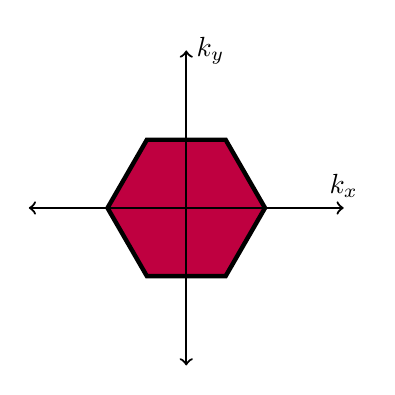
\begin{tikzpicture}
\path [fill=purple] (1,0) -- (0.5,0.866) -- (-0.5,0.866) -- (-1,0) -- (-0.5,-0.866) -- (0.5,-0.866) -- (1,0);
\draw [ultra thick] (1,0) -- (0.5,0.866) -- (-0.5,0.866) -- (-1,0) -- (-0.5,-0.866) -- (0.5,-0.866) -- (1,0);
\draw [thick,<->] (-2,0) -- (2,0) node[anchor=south ] {$k_x$};
\draw [thick,<->] (0,-2)--(0,2) node [anchor= west] {$k_y$};
\end{tikzpicture}
\caption{Brillouin zone for a hexagonal lattice. The hexagon's side lengths are $\pi/ c$, where $c$ is the lattice constant.}
\end{figure}

Without going through much of the detail of the previous simple example, the free energy of our hexagonal lattice is
\[ F = \frac{k_BTV}{8\pi^2} \int d\bv k \, \paren{ \log 64 + 2\log \paren{\lam^2 \b} + \log\paren{\eth^2 \b} + \log A^2 + \log \paren{\g_{xx} \g_{yy} - \g_{xy}^2} + \log \paren{D\mu + E\g} } .\]
Here, since one of our degrees of freedom is an angle, we don't have the thermal de Broglie wavelength, but rather a thermal de Broglie angle:
\[ \eth = \sqrt{\frac{h^2}{2\pi I k_BT}}.\]
We can do a change of variables, $\bv u = \half{ \bv k c}$, which pulls out a factor of $\frac{4}{c^2}$ from the integral. Furthermore, since we're only interested in the parts of the free energy that are dependent on the volume, we can remove the numerical factors like $\log 64$ and the thermal factors $\log \lam^2 \b$ and $\log \eth^2 \b$. The term $\log \paren{\g_{xx}\g_{yy} - \g_{xy}^2}$ integrates to some numerical constant over the Brillouin zone, as well, so we can remove it from the integral. The term $\log A^2$ can be integrated over the Brillouin zone immediately, since it doesn't depend on $\bv k$. That leaves just the last term:
\[ F_V = \frac{k_BTN}{\pi^2}\paren{\frac{3\sqrt{3} \pi^2}{8}\log A} + \frac{k_BTN}{2\pi^2} \int d\bv u \, \log \paren{D\mu + E\g}.\]
\[ F_V = \frac{3k_BT N \sqrt{3}}{8}\log A + \frac{k_BTN}{2\pi^2} \int d\bv u\, \log \paren{D\mu + E\g}.\]
\[ \g = \sin^2u_x + \sin^2\paren{\half{u_x+\sqrt{3} u_y}} + \sin^2 \paren{\half{u_x - \sqrt{3}u_y}}.\]
\[ \mu = \cos^2u_x + \cos^2\paren{\half{u_x+\sqrt{3} u_y}} + \cos^2 \paren{\half{u_x - \sqrt{3}u_y}}.\]
Both $\g$ and $\mu$ are symmetric if we rotate $\bv u$ by $\pi/3$, so instead of integrating over the whole Brillouin zone, we can just integrate over one sixth of the Brillouin zone. However we're better served by integrating over a \emph{third} of the Brillouin zone and multiplying by 3, because this gives us a rhombic region to integrate, which is far easier to do using two integration variables. Define
\[ u_x = \half{\th_1 + \th_2},\qquad u_y = \half{\sqrt{3}(\th_1-\th_2)}.\]
Then the $\th$ variables range from $0\goto \pi/2$. This change of variables is shown in Figure 2. Then $\g$ becomes
\[ \g = \sin^2\paren{\half{\th_1+\th_2}} + \sin^2 \paren{\half{2\th_1 - \th_2}} + \sin^2 \paren{\half{\th_1 - 2\th_2}},\]
and $\mu$ is defined similarly.

\begin{figure}
\centering
\begin{tikzpicture}
\path [fill=purple] (1,0) -- (0.5,0.866) -- (0,0) -- (0.5,-0.866) -- (1,0);
\draw [ultra thick] (1,0) -- (0.5,0.866) -- (-0.5,0.866) -- (-1,0) -- (-0.5,-0.866) -- (0.5,-0.866) -- (1,0);
\draw [thick,<->] (-2,0) -- (2,0) node[anchor=south ] {$u_x$};
\draw [thick,<->] (0,-2)--(0,2) node [anchor= west] {$u_y$};
\draw [thick,->] (0,0)--(0.7,1.212) node [anchor = west] {$\th_1$};
\draw [thick,->] (0,0)--(0.7,-1.212) node [anchor = west] {$\th_2$};
\end{tikzpicture}
\caption{Integrating over a third of the first Brillouin zone using some transformed variables.}
\end{figure}
Gathering all this together:
\[ F_V = \frac{3k_BTN\sqrt{3}}{8}\log A + 3\times \frac{k_BTN\sqrt{3}}{4\pi^2} \int_0^{\pi/2}\int_0^{\pi/2}d\th_1 d\th_2 \, \log\paren{D\mu + E\g}.\]
To get the pressure, we derive with respect to the volume. But what is more useful and intuitive is to derive with respect to the packing fraction, where
\[ \phi = \frac{Nv_0}{V}.\]
\[ \pder{}{V} = \pder{\phi}{V}\pder{}{\phi} = -\frac{Nv_0}{V^2}\pder{}{\phi} = -\frac{\phi^2}{Nv_0}\pder{}{\phi}.\]
\[ P = -\pder{F_V}{V} = \frac{\phi^2}{Nv_0}\pder{F_V}{\phi}.\]
Now let's define the dimensionless parameter $\e = E/D$, which is experimentally shown to be small. If we denote derivatives with respect to packing fraction as $A' = \pder{A}{\phi}$, then with a little manipulation, our pressure becomes
\[ P = \frac{3k_BT\phi^2A'\sqrt{3}}{8Av_0} + \frac{3k_BT\phi^2 E'\sqrt{3}}{16Ev_0} + \frac{3k_BT\phi^2 \e'\sqrt{3}}{4\pi^2v_0}\int_0^{\pi/2}\int_0^{\pi/2}d\th_1d\th_2\, \frac{\mu}{\e\mu+\g}.\]
\[ P = \frac{3k_BT\phi^2\sqrt{3}}{16v_0} \paren{ \frac{2A'}{A} + \frac{E'}{E} + \e' h(\e)}.\]
\[ h(\e) = \frac{4}{\pi^2} \int_0^{\pi/2}\int_0^{\pi/2}d\th_1d\th_2\, \frac{\mu}{\e\mu+\g}, \qquad \e = \frac{D}{E}, \qquad \e' = \frac{D'}{E} - \frac{DE'}{E^2}.\]
Because $\g(\th_1=\th_2=0) \propto \th_1^2 + \th_2^2$, but $\mu \propto 1$ there is a logarithmic divergence at the origin unless $\e\neq 0$. As it stands, I believe this integral is intractable. Furthermore, an expansion in $\e$ is no good, because the very first term of the series diverges, and every following term is more severely divergent. If anybody has a good idea where to go from here, that'd be great.

%However, we can do some gleaning about the equation of state based on the assumption that the coupling constants $E$ and $D$ depend on the packing fraction $\phi$. In the traditional spirit surrounding critical phenomena, I'm going to make the assumption that these parameters go to 0 as a power law as we approach the critical density (densities):
%\[ E = E_0 (\phi-\phi_E)^{\nu_E},\qquad D = D_0 (\phi-\phi_D)^{\nu_D}, \qquad \e = \frac{D_0}{E_0}\frac{(\phi-\phi_D)^{\nu_D}}{(\phi-\phi_E)^{\nu_E}}.\]
%We don't have much information about the critical densities or the critical exponents (besides that they are both greater than 0), but we can discern a few different cases. First, $\phi_E = \phi_D$ or $\phi_E \neq \phi_D$. Then, we have the case that $\nu_E > \nu_D$, $\nu_E = \nu_D$, or $\nu_E < \nu_D$. First, I'll explore what happens when $\phi_E = \phi_D$, so that
%\[ \e = \e_0 (\phi - \phi_c)^{\nu_D - \nu_E}, \qquad \e' = \e_0 (\phi-\phi_c)^{\nu_D-\nu_E - 1}.\]
%In this case,
%\[ P = \frac{3k_BT\phi^2\sqrt{3}}{16v_0}\paren{\frac{2A'}{A} + (\phi-\phi_c)^{-1} + (\phi-\phi_c)^{-1} \paren{ \e h(\e)}}.\]


\section{Complex Unit Cells and Optical Libron Bands}

\subsection{Toy Model: 1D Chain Revisited}

Here, we'll revamp the 1D chain so we have two atoms of different types 
supporting two degrees of freedom each, $a$ and $b$. The atoms will be labeled 
$\a$ and $\b$, and there is one atom of each type in each unit cell. The 
distance between $\a$ and $\b$ particles of the same cell is $c_1$, and the 
distance between $\a$ and $\b$ particles of differing unit cells is $c_2$. 
Figure \ref{1dchain2} illustrates the situation.

\begin{figure}
\centering
\begin{tikzpicture}

\draw (0,0) rectangle (3,1);
\draw (3,0) rectangle (6,1);
\draw (6,0) rectangle (9,1);
\draw [color=blue,fill] (1,0.5) circle (0.3);
\draw [color=purple,fill] (2,0.5) circle (0.2);
\draw [color=blue,fill] (4,0.5) circle (0.3);
\draw [color=purple,fill] (5,0.5) circle (0.2);
\draw [color=blue,fill] (7,0.5) circle (0.3);
\draw [color=purple,fill] (8,0.5) circle (0.2);
\draw [dashed] (1,0.5) -- (2,0.5);
\draw [dashed] (5,0.5) -- (7,0.5);
\draw (1.5,0.5) node [anchor=south] {$c_1$};
\draw (6,0.5) node [anchor=south east] {$c_2$};
\draw (0.4,0.5) node {$\a$};
\draw (2.5,0.5) node {$\b$};
\draw (1.5,0) [anchor=north] node {$i-1$};
\draw (4.5,0) [anchor=north] node {$i$};
\draw (7.5,0) [anchor=north] node {$i+1$};
\end{tikzpicture}
\caption{Intricate field interactions for many-particle unit cells.}
\label{1dchain2}
\end{figure}

The interactions between the fields that live on neighboring atoms will contain 
terms that look like $(a^\a_i - a^\b_i)^2$ and $(a^\b_{i-1} - 
a^\a_i)(b^\b_{i-1} - b^\a_i)$, and all of these terms will have different 
coupling constants. We could use a matrix equation to describe the interaction 
energy of the $c_1$ bond between atoms of cell $i$:
\[ U_{c_1,i} = \half{1} \pmtrx{a^\a_i - a^\b_i & b^\a_i - b^\b_i}
 \pmtrx{K_{aa} & K_{ab} \\ K_{ab} & K_{bb}} \pmtrx{a^\a_i - a^\b_i \\ b^\a_i - 
b^\b_i}.\]
The matrix $\bv K$ must necessarily be symmetric. The $U_{c_2,i}$ term which bonds 
the $\b$ atom of cell $i-1$ and the $\a$ atom of cell $i$ looks similar, but in 
general, with a different coupling constant matrix:
\[ U_{c_2,i} = \half{1} \pmtrx{a^\b_{i-1} - a^\a_i & b^\b_{i-1} - b^\a_i}
 \pmtrx{M_{aa} & M_{ab} \\ M_{ab} & M_{bb}} \pmtrx{a^\b_{i-1} - a^\a_i & 
b^\b_{i-1} - b^\a_i}.\]
So the total energy $U$ is the sum over the $i$ cells of these two terms. It's 
important to note that since the only terms that appear in the energy are 
\emph{differences} in the field values $a$ and $b$, this theory will only 
generate \emph{massless} modes, as opposed to the very first example I 
provided where I put in a mass by hand. The mass is produced by the breaking of 
translational invariance, but here, I'm maintaining translational invariance by 
supposing the energy is only a function of differences in field values.

It is easiest, in fact, to perform the Fourier transform here and now before 
proceeding to derive the equations of motion. We should use the same convention 
FT that we used in previous problems: $u_i=\recip{\sqrt{N}} \sum_k 
\tilde{u}_k e^{-ikr_i}$, where $u_i$ is any field. Inserting the Fourier 
transformed fields into the expression for energy of the $c_1$ type bonds:
\begin{multline*} U_{c_1} = \half{1} \recip{N} \sum_i \sum_k \sum_{k'}  
\pmtrx{\tilde a^\a_{k'} e^{-ik'r_i} - \tilde a^\b_{k'} e^{-ik'r_i - ik'c_1} & 
\tilde b^\a_{k'} e^{-ik'r_i} - \tilde b^\b_{k'} e^{-ik'r_i - ik'c_1}} \cdot \\
 \pmtrx{K_{aa} & K_{ab} \\ K_{ab} & K_{bb}}  \pmtrx{\tilde a^\a_{k} 
e^{-ikr_i} - \tilde a^\b_{k} e^{-ikr_i - ikc_1} \\
\tilde b^\a_{k} e^{-ikr_i} - \tilde b^\b_{k} e^{-ikr_i - ikc_1}}. 
\end{multline*}
Or, to make things a bit cleaner, we can pull out exponential factors from 
everywhere:
\begin{multline*} U_{c_1} = \half{1} \recip{N} \sum_i \sum_k \sum_{k'}  
e^{-ik'r_i -ikr_i}
\pmtrx{\tilde a^\a_{k'}  - \tilde a^\b_{k'} e^{- ik'c_1} & 
\tilde b^\a_{k'} - \tilde b^\b_{k'} e^{- ik'c_1}}
 \pmtrx{K_{aa} & K_{ab} \\ K_{ab} & K_{bb}}  \pmtrx{\tilde a^\a_{k} 
 - \tilde a^\b_{k} e^{- ikc_1} \\
\tilde b^\a_{k} - \tilde b^\b_{k} e^{- ikc_1}}. 
\end{multline*}
The sum over $i$ produces 0 unless the argument of the exponential out in 
front, $(k+k')r_i$ vanishes, which implies $k = -k'$. The sum over $i$ in this 
case produces a factor of $N$, which nicely cancels the Fourier transform 
normalization, and then we can perform the sum over $k'$:
\[ U_{c_1} = \half{1} \sum_{k} 
\pmtrx{\tilde a^\a_{-k}  - \tilde a^\b_{-k} e^{ikc_1} & 
\tilde b^\a_{-k} - \tilde b^\b_{-k} e^{ikc_1}}
 \pmtrx{K_{aa} & K_{ab} \\ K_{ab} & K_{bb}}  \pmtrx{\tilde a^\a_{k} 
 - \tilde a^\b_{k} e^{- ikc_1} \\
\tilde b^\a_{k} - \tilde b^\b_{k} e^{- ikc_1}}.\]
Likewise, for the $U_{c_2}$ term,
\[ U_{c_2} = \half{1} \sum_{k} 
\pmtrx{\tilde a^\a_{-k}  - \tilde a^\b_{-k} e^{-ikc_2} & 
\tilde b^\a_{-k} - \tilde b^\b_{-k} e^{-ikc_2}}
 \pmtrx{M_{aa} & M_{ab} \\ M_{ab} & M_{bb}}  \pmtrx{\tilde a^\a_{k} 
 - \tilde a^\b_{k} e^{ ikc_2} \\
\tilde b^\a_{k} - \tilde b^\b_{k} e^{ ikc_2}}.\]
Instead of writing these energies in terms of the 2-component vector of 
differences, we could write everything in terms of a 4-component vector of the 
field values:
\[ U_{c_1} = \pmtrx{\tilde a^\a_{-k} & \tilde b^\a_{-k} & \tilde a^\b_{-k} & 
\tilde b^\b_{-k}} \pmtrx{ K_{aa} & K_{ab} & -K_{aa} e^{-ikc_1} & -K_{ab} 
e^{-ikc_1} \\
K_{ab} & K_{bb} & -K_{ab}e^{-ikc_1} & -K_{bb}e^{-ikc_1} \\ -K_{aa} e^{ikc_1} & 
-K_{ab} e^{ikc_1} & K_{aa} & K_{ab} \\ -K_{ab} e^{ikc_1} & -K_{bb}e^{ikc_1} 
& K_{ab} & K_{bb} } \pmtrx{\tilde a^\a_k \\ \tilde b^\a_k \\ \tilde a^\b_k \\ 
\tilde b^\b_k}.\]
Similarly:
\[ U_{c_2} = \pmtrx{\tilde a^\a_{-k} & \tilde b^\a_{-k} & \tilde a^\b_{-k} & 
\tilde b^\b_{-k}} \pmtrx{ M_{aa} & M_{ab} & -M_{aa} e^{ikc_2} & -M_{ab} 
e^{ikc_2} \\
M_{ab} & M_{bb} & -M_{ab}e^{ikc_2} & -M_{bb}e^{ikc_2} \\ -M_{aa} e^{-ikc_2} & 
-M_{ab} e^{-ikc_2} & M_{aa} & M_{ab} \\ -M_{ab} e^{-ikc_2} & -M_{bb}e^{-ikc_2} 
& M_{ab} & M_{bb} } \pmtrx{\tilde a^\a_k \\ \tilde b^\a_k \\ \tilde a^\b_k \\ 
\tilde b^\b_k}.\]
If we define the fields at atom $\a$ by $\bv u^\a = \paren{ a^\a, b^\a}$ and 
the fields at atom $\b$ similarly, we can formulate the energies quite simply:
\[ U = \half{1} \sum_k \pmtrx{ \bv{\tilde u}^\a_{-k} & \bv{\tilde u}^\b_{-k}} 
\pmtrx{ \bv K + \bv M & - \bv K e^{-ikc_1} - \bv Me^{ikc_2} \\ - \bv Ke^{ikc_1} - \bv Me^{-ikc_2} & 
\bv K+\bv M} \pmtrx{ \bv{\tilde u}^\a_k \\ \bv{\tilde u}^\b_k }.\]
Here, $\bv K$ and $\bv M$ are the full matrices, not components of the matrices. The 
next useful step is to replace $\bv{\tilde u}_{-k}$ with $\bv{\tilde u}_k^*$, 
the complex conjugate, which is a property of the Fourier transform of real 
fields $\bv u_i$. By summing over all of $k$, we're actually double-counting, 
because the modes of opposite wavenumber are connected in this way, that is, 
$\bv{\tilde u}_{-k} = \bv{\tilde u}_k^*$.

It's at this point that we need to derive the equations of motion, but first, 
I'd like to clarify a technical but important detail with a brief example.

\subsubsection{Complex degrees of freedom}
Consider a 2D harmonic oscillator, whose Lagrangian is
\[ \mathcal{L} = \half{1} \paren{ \dot x ^2 + \dot y^2} - \half{1} \w_0^2 
\paren{x^2 + y^2}.\]
Here, I've set the mass equal to one for simplicity. The equations 
of motion are very simple, they come from the Euler-Lagrange equations:
\[ \der{}{t} \pder{\mathcal L}{\dot x} = \pder{\mathcal L}{x}, \qquad \der{}{t} 
\pder{\mathcal L} {\dot y} = \pder{\mathcal L}{y}.\]
\[ \der{}{t} \paren{\dot x} = -\w_0^2 x, \qquad \der{}{t} \paren{\dot y} = 
-\w_0^2 y.\]
\[ \ddot x = -\w_0^2 x, \qquad \ddot y = -\w_0^2 y.\]
Another way to write the Lagrangian is by defining the complex degrees of 
freedom:
\[ z = \frac{x+iy}{\sqrt{2}} ,\qquad z^* = \frac{x-iy}{\sqrt 2}.\]
Then the Lagrangian can be written succinctly as
\[ \mathcal L = \dot z \dot z^* - \w_0^2 z z^*.\]
So the Euler-Lagrange equations give us:
\[ \der{}t\paren{ \dot z^* } = -\w_0^2 z^*, \qquad \der{}t\paren{ \dot z} = 
-\w_0^2 z.\]
\[ \ddot z^* = -\w_0^2 z^*, \qquad \ddot z = -\w_0^2 z.\]
In terms of the modes of the harmonic oscillator, a wave in the variables $x$ 
and $y$ are linearly polarized waves. The interpretation of $z$ and $z^*$ are 
then circularly polarized wave modes. Notice that we included the $\sqrt{2}$ in 
the definition of $z$ and $z^*$. Had we used some other normalization (or even 
different normalizations), the results would've been identical. Let's define 
instead:
\[ w = C_1(x+iy),\qquad w^* = C_2(x-iy).\]
Then the Lagrangian is
\[ \mathcal L = \recip{2 C_1 C_2} \dot w \dot w^* - \recip{2C_1 C_2}\w_0^2 w 
w^*.\]
The Euler-Lagrange equations produce the same thing:
\[ \ddot w^* = -\w_0^2 w^*, \qquad \ddot w = -\w_0^2 w.\]
Notice that $w$ and $w^*$ are \emph{not} complex conjugates of one another. 
They are \emph{separate, independent degrees of freedom.} This has to be the 
case, because the original system had two degrees of freedom, any 
reparameterization should also have two independent degrees of freedom, as 
well.

\hrulefill

Returning to the derivation for the 1D chain, we have again:
\[ U = \half{1} \sum_k \pmtrx{ \bv{\tilde u}^\a_{-k} & \bv{\tilde u}^\b_{-k}} 
\pmtrx{ \bv K + \bv M & - \bv K e^{-ikc_1} - \bv Me^{ikc_2} \\ - \bv Ke^{ikc_1} - \bv Me^{-ikc_2} & 
\bv K+\bv M} \pmtrx{ \bv{\tilde u}^\a_k \\ \bv{\tilde u}^\b_k }.\]
The sum over $k$ is over the entire Brillouin zone. However, we note that this 
sum is necessarily symmetric about $k=0$. Instead of summing over $k$ from 
$-\pi/(c_1+c_2)N$ to $\pi/(c_1+c_2)N$, we can just sum the $k\geq0$ twice. This 
eliminates the $1/2$, and we write $\bv{\tilde u}_{-k}$ instead as $\bv{\tilde
u}_{k}^*$. Our Lagrangian is then
\[ \mathcal{L} = \sum_{k\geq 0} \pmtrx{ \bv{\dot{\tilde u}}^{\a *}_{k} & 
\bv{\dot{\tilde u}}^{\b *}_{k}} \cdot \pmtrx{ \bv{\dot{\tilde u}}^\a_k \\ 
\bv{\dot{\tilde u}}^\b_k } - 
\pmtrx{ \bv{\tilde u}^{\a *}_{k} & \bv{\tilde 
u}^{\b *}_{k}} \pmtrx{ \bv K + \bv M & - \bv K e^{-ikc_1} - \bv 
Me^{ikc_2} \\ - \bv Ke^{ikc_1} - 
\bv Me^{-ikc_2} & \bv K+\bv M} \pmtrx{ \bv{\tilde u}^\a_k \\ \bv{\tilde 
u}^\b_k }.\]
Just as in the demonstrative example above, the Euler-Lagrange equations 
furnish the equations of motion with the right factors of $1/2$ missing and 
such:
\[ \der{}{t} \paren{ \pder{\mathcal{L}}{\pmtrx{ \bv{\dot{\tilde u}}^{\a *}_{k} 
& 
\bv{\dot{\tilde u}}^{\b *}_{k}} } } = \pder{\mathcal{L}}{ \pmtrx{ \bv{\tilde 
u}^{\a *}_{k} & \bv{\tilde 
u}^{\b *}_{k}} }.\]
\[ \pmtrx{ \bv{\ddot{\tilde u}}^\a_k \\ \bv{\ddot{\tilde u}}^\b_k } = -\pmtrx{ 
\bv K + \bv M & - \bv K e^{-ikc_1} - \bv Me^{ikc_2} \\ - \bv Ke^{ikc_1} - 
\bv Me^{-ikc_2} & \bv K+\bv M} \pmtrx{ \bv{\tilde u}^\a_k \\ \bv{\tilde u}^\b_k }.\]
Then going to frequency space:
\[ \w^2 \pmtrx{ \bv{\tilde u}^\a_k \\ \bv{\tilde u}^\b_k } = 
\pmtrx{ 
\bv K + \bv M & - \bv K e^{-ikc_1} - \bv Me^{ikc_2} \\ - \bv Ke^{ikc_1} - 
\bv Me^{-ikc_2} & \bv K+\bv M} \pmtrx{ \bv{\tilde u}^\a_k \\ \bv{\tilde u}^\b_k }.\]
Here, $\bv K$ and $\bv M$ are the coupling matrices between the field $\tilde a$ and 
$\tilde b$, and they are embedded in a larger matrix that encodes the spatial 
information of how atoms are organized and which atoms are coupled to which. 
The set of $\a$ fields $\bv{\tilde u}^\a$ is coupled to the set of $\b$ 
fields $\bv{\tilde u}^\b$ with a term like $-\bv K e^{-ikc_1} -\bv M e^{+ikc_2}$. 
The first term couples the $\a$ fields to the $\b$ fields a 
distance $c_1$ to the right using the matrix of spring constants $\bv K$ and, and 
the second term couples the $\a$ fields to the $\b$ fields to the left a 
distance $c_2$ using the matrix of spring constants $\bv M$.

In this formulation, the generalization to two dimensions is straightforward: 
the only substitution to be made is $kc \goto \Dot kc$. Furthermore, we've 
teased out the structure of the master coupling matrix, which is in general has 
size $nf \times nf $, where $n$ is the number of particles in the 
unit cell and $f$ is the number of fields per particle. This big matrix is a 
$n\times n$ matrix whose components themselves are $f\times f$ matrices.


\subsection{Pentagon Crystal Modes}

The densest packing of the pentagon crystal is a rectangular Bravais lattice whose unit cells contain two antiparallel pentagons. The parametrization of the crystal I'm using in my simulations and the one I'll be using in this analysis relies on the following parameters of the densest packing structure (shown in Figure \ref{pentcrystal}):
\begin{center}
\def\arraystretch{1.2}
\begin{tabular}{|c|c|c|c|} \hline
Vector & Symbol & Value\\ \hline
Short real-space lattice vector & $\bv a_1$ & $\half{1} \paren{1+\cos \frac{\pi}{5}}\hat x $\\ \hline
Long real-space lattice vector & $\bv a_2$ &$ \half{3} \sin\frac{2\pi}{5} \hat y $\\ \hline
Location of right-facing pentagon in unit cell& & $0$ \\ \hline
Location of left-facing pentagon in unit cell& $\bv p$ & $\paren{\recip{4} + \frac{3}{4} \cos \frac{2\pi}{5} } \hat x + \frac{3}{4}\sin\frac{2\pi}{5} \hat y$  \\ \hline
\end{tabular}
\end{center}

\begin{figure}
\centering
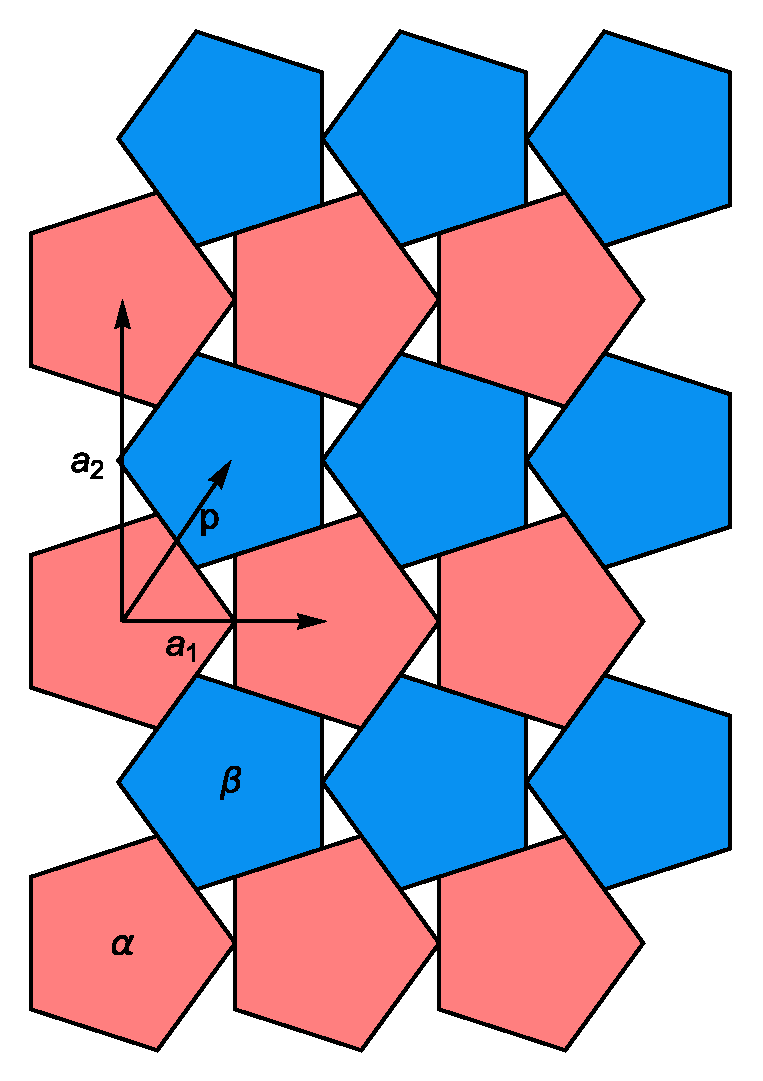
\includegraphics[scale=0.6]{pentagons.eps}
\caption{Unproven pentagon densest packing. A magenta pentagon ($\a$ particle) and the blue pentagon ($\b$ particle) to its upper-right comprise the unit cell in this analysis. The vector going from the magenta to the blue pentagon is $\bv p$, the vector between pentagons in a row is $\bv a_1$, and the vector between pentagons in the same column is $\bv a_2$.}
\label{pentcrystal}
\end{figure}

Now, we need to characterize the various matrices that couple the modes of each pentagon to each other. As before with the hexagons (page 5), we characterize the relevant degrees of freedom:
\[ \bv v_{\br,\bv c} = \paren{ \paren{u_{x,\br} - u_{x,\br + \bv c}}\hat c_x, \paren{ u_{y,\br} - u_{y,\br + \bv c} } \hat c_y, \th_\br + \th_{\br + \bv c}, \th_\br - \th_{\br + \bv c} },\]
and the general matrix that couples the pentagons' degrees of freedom looks like:
\[ \bv M = \pmtrx{ A & A & B & C \\ A & A & B & C \\ B & B & D & F \\ C & C & F & E},\]
so that the quadratic energy that characterizes an interaction between a pentagon and its neighbor separated by nearest-neighbor vector $\bv c$ is
\[ U_{\br, \bv c} = \half{1} v_iM_{ij}v_j.\]
The beautiful thing (which I didn't realize while doing the hexagon lattice) is that the coupling constants $B$ and $C$ must necessarily be 0. The reason is because of the inversion symmetry of interactions between 2D particles (not of the lattice!). If we take two pentagons and invert them across the $y$-axis, for example, the first two components of $\bv v$ are invariant ($u_x$ changes sign but so does $\hat c_x$, and $u_y$ and $\hat c_y$ are left invariant separately); the displacement degrees of freedom are \emph{even under inversion}. However, the pentagons' $\th$ degree of freedom (or to be more explicit, their angular displacement relative to an equilibrium angle), is swept out \emph{in the opposite direction}, so $\th \goto -\th$; the $\th$ degree of freedom is \emph{odd under inversion}. Because $U$ itself must be even under inversion, terms involving the product of one even and one odd degree of freedom cannot appear in $U$. Therefore, $B=C=0$ in the coupling matrix $\bv M$. In general, the constant $F$ can still be nonzero. In the hexagon crystal, $F$ vanished because of the complete inversion symmetry \emph{of the whole lattice}. In the triangular lattice, for every $\bv c$, there is an exact opposite $-\bv c$, and $F$ represented terms that got cancelled exactly when we summed over all six neighbors. Here in the pentagon crystal, this isn't the case, so we need to keep $F$.

It's important to note that while terms coupling $\th$ and $\hat c \cdot \bv u$ cannot appear in $U$ to quadratic order, these degrees of freedom are coupled by \emph{cubic} terms. Because $\th^2$ is invariant under inversion symmetry, the smallest polynomial we can make that is even all together is $(\th^2) (\hat c \cdot \bv u)$, which is a cubic term.

\begin{figure}
\centering
\begin{subfigure}{0.4\textwidth}
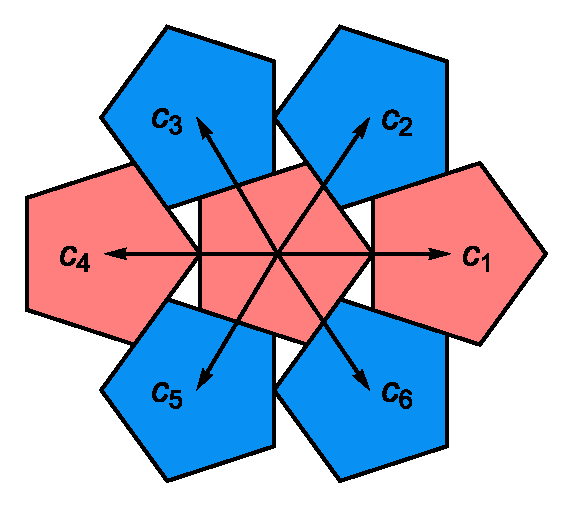
\includegraphics[scale=0.6]{alphabonds.eps}
\end{subfigure}
\begin{subfigure}{0.4\textwidth}
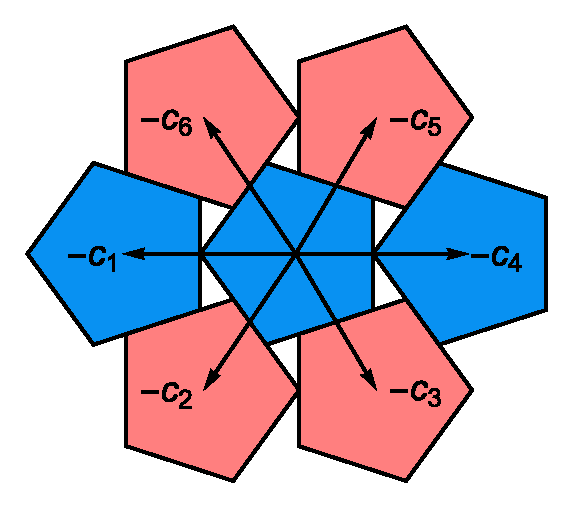
\includegraphics[scale=0.6]{betabonds.eps}
\end{subfigure}
\caption{The nearest neighbor configurations of $\a$ particles (left) and $\b$ 
particles (right). The nearest neighbor vectors are related to each other by a 
$\pi$ rotation. Further symmetries constrain the components of the set of $\bv 
c$: $\bv c_1 = -\bv c_4$, $c_{2,x} = c_{6,x}$, $c_{2,y}=-c_{6,y}$, $c_{3,x} = 
c_{5,x}$, and $c_{3,y} = -c_{5,y}$. The configuration is very nearly hexagonal, 
but the 6-fold symmetry is slightly broken into a 2-fold symmetry. To be 
explicit, the angle between $\bv c_1$ and $\bv c_2$ is $55.965^\circ$, the angle 
between $\bv c_2$ and $\bv c_3$ is $64.689^\circ$, and the angle between $\bv 
c_3$ and $\bv c_4$ is $59.346^\circ$.}
\label{pentagonnn}
\end{figure}

There are three distinct bond types, characterized by the vectors $\bv c_{1,2,3}$, and the bonds characterized by $\bv c_{4,5,6}$ are related exactly by symmetry. In the toy model we considered previously, we had two bond types, which we characterized by two coupling matrices $\bv K$ and $\bv M$. Here we'll need three separate matrices to describe each of these bonds, and they will all look like the matrix $\bv M$ defined above (but with $B=C=0$). I'll write these different $\bv M$ matrices with a subscript $\bv M_{a=1,2,3}$.

Now, let's write down the energy of bond $\bv c_1$, for example:
\[ U_{\bv c_1,i} = \half{1} \bv v_{\br_i, \bv c_1} \cdot \bv M_1 \cdot \bv 
v_{\br_i,\bv c_1}.\]
The elements of $\bv M_1$ are $A_1,D_1,E_1,$ and $F_1$. We perform the Fourier transform on $\bv v_{\br_i,\bv c_1}$:
\[ \bv{\tilde v}_{\bv k,\bv c_1} = \paren{ \hat c_{1,x}\tilde u_{x,\bv k}^\a 
\paren{1-e^{-i\Dot{k}{c_1}}}, \, \hat c_{1,y}\tilde u_{y,\bv 
k}^\a\paren{1-e^{-i\Dot{k}{c_1}}}, \, \tilde \th_{\bv k}^\a 
\paren{1+e^{-i\Dot{k}{c_1} } }, \, \tilde \th_{\bv k}^\a 
\paren{1-e^{-i\Dot{k}{c_1} } }   }.\]

Performing the matrix product, we can make a new matrix of just the field 
values, not their differences or sums:
\begin{multline*} U_{\bv c_1,\bv k} = \half{1} \paren{\tilde u^{\a *}_{x,\bv 
k}, \, \tilde u^{\a *}_{y,\bv k},\, \tilde \th^{\a *}_{\bv k}} \cdot \\ \pmtrx{ 
4A_1 \hat c_{1,x}^2 \sin^2\half{\Dot{k}{c_1}} & 4A_1 \hat 
c_{1,x} \hat c_{1,y} \sin^2\half{\Dot{k}{c_1}} & 0 \\ 4A_1 \hat 
c_{1,x} \hat c_{1,y} \sin^2\half{\Dot{k}{c_1}} & 4A_1 \hat 
c_{1,y}^2 \sin^2\half{\Dot{k}{c_1}} & 0 \\ 0 & 0 & 4D_1\cos^2 
\half{\Dot{k}{c_1}} + 4E_1 \sin^2 \half{\Dot{k}{c_1}} } \pmtrx{ \tilde 
u^\a_{x,\bv k} \\ \tilde u^\a_{y,\bv k} \\ \tilde \th^\a_{\bv k} 
}.\end{multline*}
Here we see again that the $F_1$ term has dropped out. Also note, that this 
term in the energy does not contain any $\b$ fields, because this energy is 
the bond energy between two $\a$ particles. Now, let's perform the same 
analysis of the energy for the bond spanned by $\bv c_2$ that joins an $\a$ 
particle with a $\b$ particle. Here, the matrix will be larger dimensional. 
This time, the vector $\bv v_{\bv r_i,\bv c_2}$ contains both $\a$ and $\b$ 
fields. Also, for all our sanity, I'm going to drop the $\bv k$ subscript, and 
assume that these Fourier modes take a wavevector argument.
\[ \bv v_{\bv r_i, \bv c_2} = \paren{ \hat c_{2,x}\paren{\tilde u_x^\a- 
\tilde u_x^\b e^{-i\Dot{k}{c_2}}}, \, \hat c_{2,y}\paren{\tilde 
u_y^\a-\tilde u_y^\b e^{-i\Dot{k}{c_2}}}, \, \tilde \th^\a +
\tilde \th^\b e^{-i\Dot{k}{c_2}}, \, \tilde \th^\a -\tilde 
\th^\b e^{-i\Dot{k}{c_2} } }.\]
\begin{multline*} U_{\bv c_2} = \half{1} \paren{\tilde u_x^{\a *} 
, \, \tilde 
u_y^{\a *} , \, \tilde \th^{\a *} , \, \tilde u_x^{\b *} , \, \tilde u_y^{\b *}, 
\, \tilde \th^{\b *} } \cdot \\  \pmtrx{
 A_2\bv C_2 & 0 & -A_2 \bv C_2 e^{-i\Dot{k}{c_2}} & 0 \\
0 & D_2 + 2F_2 + E_2 & 0 & D_2e^{-i\Dot{k}{c_2}} - 
E_2e^{-i\Dot{k}{c_2}} \\
-A_2 \bv C_2 e^{i\Dot{k}{c_2}} & 0 & A_2 \bv C_2 & 0  \\
0 &  D_2 e^{i\Dot{k}{c_2}} - E_2 e^{i\Dot{k}{c_2}} & 0  & D_2 - 2F_2 + 
E_2}
\pmtrx{\tilde u_x^{\a} \\ \tilde 
u_y^{\a} \\ \tilde \th^{\a} \\ \tilde u_x^{\b} \\ \tilde u_y^{\b} \\  \tilde 
\th^{\b} }.\end{multline*}
Here, for the sake of fitting the whole equation within the margins, the 
$2\times 2$ matrix $\bv C_2$ is defined as the outer product of the vector $\bv 
c_2$ with itself
\[ \bv C_2 = \pmtrx{ \hat c_{2,x}^2 & \hat c_{2,x}\hat c_{2,y} \\ \hat 
c_{2,x}\hat c_{2,y} & \hat c_{2,y}^2 }.\]
We need one term in the energy for every wavevector $\bv k$ and for every kind 
of distinct bond $\bv c_i$. We need to be careful which bonds we count because 
some are related just by a translation by a lattice vector. For example, we 
already counted the bond between two $\a$ particles spanned by $\bv c_1$, but 
we should not count a term between two $\a$ particles spanned by $\bv c_4$, 
because this bond is related to the first bond by a translation by $\bv a_1$. 
However, we \emph{do} need to count the bond spanned by $\bv c_1$ that joins 
two $\b$ \emph{particles} together, because this bond is related to the 
$\a$-$\a$ bond by the vector $\bv p$, which isn't a lattice vector but a vector 
characteristic of the unit cell. To make sure we tile all of bond space with 
the right number of bonds without overlap, we need \emph{six} terms. To 
illustrate, refer to Figure \ref{pentagonnn}. The first three bonds are the 
$\a$-$\a$ bond by $\bv c_1$, the $\a$-$\b$ bond by $\bv c_2$, and the $\a$-$\b$ 
bond by $\bv c_3$, which are shown in the left subfigure. The second set of 
three bonds (right subfigure) are the $\b$-$\b$ bond by $-\bv c_4$, the 
$\b$-$\a$ bond by $-\bv c_5$, and the $\b$-$\a$ bond by $-\bv c_6$. The 
potential energy at wavevector $\bv k$ is thus
\[ U_{\bv k} = \half{1} \paren{\tilde {\bv u}^{\a *} 
, \, \tilde \th^{\a *} , \, \tilde {\bv u}^{\b *} , \, \tilde \th^{\b *} }\cdot 
\paren{ \sum_{i=1\ldots 6} \bv K_i } \cdot \pmtrx{\tilde {\bv u}^{\a} \\ \tilde 
\th^{\a} \\ \tilde {\bv u}^{\b} \\  \tilde \th^{\b} }.\]
And the six matrices $\bv K_i$ are the following:
\[ \bv K_1 = \pmtrx{ 4A_1 \bv C_1 \sin^2 \half{\Dot{k}{c_1}} & 0 & 0 & 0\\ 0 & 
4D_1 \cos^2\half{\Dot{k}{c_1}} + 4E_1 \sin^2 \half{\Dot{k}{c_1}} & 0 & 0 \\ 
0 & 0 & 0 & 0 \\ 0 & 0 & 0 & 0}.\]
\[ \bv K_2 = \pmtrx{
 A_2\bv C_2 & 0 & -A_2 \bv C_2 e^{-i\Dot{k}{c_2}} & 0 \\
0 & D_2 + 2F_2 + E_2 & 0 & D_2e^{-i\Dot{k}{c_2}} - 
E_2e^{-i\Dot{k}{c_2}} \\
-A_2 \bv C_2 e^{i\Dot{k}{c_2}} & 0 & A_2 \bv C_2 & 0  \\
0 &  D_2 e^{i\Dot{k}{c_2}} - E_2 e^{i\Dot{k}{c_2}} & 0  & D_2 - 2F_2 + 
E_2}.\]
\[ \bv K_3 = \pmtrx{
 A_3\bv C_3 & 0 & -A_3 \bv C_3 e^{-i\Dot{k}{c_3}} & 0 \\
0 & D_3 + 2F_3 + E_3 & 0 & D_3e^{-i\Dot{k}{c_3}} - 
E_3e^{-i\Dot{k}{c_3}} \\
-A_3 \bv C_3 e^{i\Dot{k}{c_3}} & 0 & A_3 \bv C_3 & 0  \\
0 &  D_3 e^{i\Dot{k}{c_3}} - E_3 e^{i\Dot{k}{c_3}} & 0  & D_3 - 2F_3 + 
E_3}.\]
\[ \bv K_4 = \pmtrx{ 0 & 0 & 0 & 0 \\ 0 & 0 & 0 & 0 \\ 0 & 0 & 4A_1 \bv C_4
\sin^2 \half{\Dot{k}{c_4}}\\ 0 & 0 & 0 & 4D_1 \cos^2\half{\Dot{k}{c_4}} + 4E_1 
\sin^2 \half{\Dot{k}{c_4}} }.\]
\[ \bv K_5 = \pmtrx{ A_3\bv C_5 & 0 & -A_3 \bv C_5 e^{-i\Dot{k}{c_5}} & 0 \\
0 & D_3 - 2F_3 + E_3 & 0 & D_3e^{-i\Dot{k}{c_5}} - 
E_3e^{-i\Dot{k}{c_5}} \\
-A_3 \bv C_5 e^{i\Dot{k}{c_5}} & 0 & A_3 \bv C_5 & 0  \\
0 &  D_3 e^{i\Dot{k}{c_5}} - E_3 e^{i\Dot{k}{c_5}} & 0  & D_3 + 2F_3 + 
E_3}.\]
\[ \bv K_6 = \pmtrx{ A_2\bv C_6 & 0 & -A_2 \bv C_6 e^{-i\Dot{k}{c_6}} & 0 \\
0 & D_2 - 2F_2 + E_2 & 0 & D_2e^{-i\Dot{k}{c_6}} - 
E_2e^{-i\Dot{k}{c_6}} \\
-A_2 \bv C_6 e^{i\Dot{k}{c_6}} & 0 & A_2 \bv C_6 & 0  \\
0 &  D_2 e^{i\Dot{k}{c_6}} - E_2 e^{i\Dot{k}{c_6}} & 0  & D_2 + 2F_2 + 
E_2}.\]
The large capital $\bv C_i$ are again the outer products of the $\bv c_i$ 
with themselves. Here, it actually makes sense to separate the phonon and 
libron degrees of freedom:
\[ U = \half{1} \paren{\tilde {\bv u}^{\a *}, \, \tilde {\bv u}^{\b *}}\cdot 
\bv K_{\bv u} \cdot \pmtrx{\tilde {\bv u}^{\a}  \\ \tilde {\bv u}^{\b}} + 
\half{1} \paren{\tilde \th^{\a *} , \, \tilde \th^{\b *} } \cdot \bv K_{\th} 
\cdot \pmtrx{ \tilde \th^\a \\ \tilde \th^\b }.\]
Where, here, these separated coupling matrices are the sums of components of 
all the $\bv K_i$ defined above. Interestingly, the terms involving $F_{2,3}$ 
cancel each other in $\bv K_\th$.
\newcommand*{\Scale}[2][4]{\scalebox{#1}{$#2$}}
\[ \Scale[0.8]{\bv K_{\bv u} = \pmtrx{ 4A_1\bv C_1 \sin^2 \half{\Dot{k}{c_1}} 
+ A_2(\bv C_2 + \bv C_6) + A_3 (\bv C_3 + \bv C_5) & -A_2\paren{ \bv C_2 
e^{-i\Dot{k}{c_2}} + \bv C_6 e^{-i\Dot{k}{c_6} }} - A_3\paren{ \bv C_3 
e^{-i\Dot{k}{c_3}} + \bv C_5 e^{-i\Dot{k}{c_5} }} \\ -A_2\paren{ \bv C_2 
e^{i\Dot{k}{c_2}} + \bv C_6 e^{i\Dot{k}{c_6} }} - A_3\paren{ \bv C_3 
e^{i\Dot{k}{c_3}} + \bv C_5 e^{i\Dot{k}{c_5} }} & 4A_1\bv C_4 \sin^2 
\half{\Dot{k}{c_4}} + 
A_2(\bv C_2 + \bv C_6) + A_3 (\bv C_3 + \bv C_5)}.}\]
\[ \Scale[0.8]{\bv K_\th = \pmtrx{ 4D_1 \cos^2 \half{\Dot{k}{c_1}} + 4E_1 
\sin^2 \half{\Dot{k}{c_1}} + 2(D_2+D_3+E_2+E_3) & 
(D_2-E_2)\paren{e^{-i\Dot{k}{c_2}} + e^{-i\Dot{k}{c_6}} } + 
(D_3-E_3)\paren{e^{-i\Dot{k}{c_3}} + e^{-i\Dot{k}{c_5}} } \\ 
(D_2-E_2)\paren{e^{i\Dot{k}{c_2}} + 
e^{i\Dot{k}{c_6}} } + (D_3-E_3)\paren{e^{i\Dot{k}{c_3}} + e^{i\Dot{k}{c_5}} 
} & 4D_1 \cos^2 \half{\Dot{k}{c_4}} + 4E_1 \sin^2 
\half{\Dot{k}{c_4}} + 2(D_2+D_3+E_2+E_3)}.}\]
We're \emph{so close.} I'd like to take a closer look at $\bv K_\th$, because 
it actually has a rather simple form. Because $\bv c_1 = -\bv c_4$, the first 
diagonal element is actually exactly equal to the second diagonal element, so 
the form of $\bv K_\th$ is
\[ \bv K_\th = \pmtrx{ x & y \\ y^* & x}.\]
This is a particularly easy matrix to diagonalize, and its eigenvalues are
\[ \w^2 = x \pm \sqrt{yy^*}.\]
The minus term will give us the acoustic libron branch, and the plus term will 
give us the optical libron branch. If we expand $x\pm \abs{y}$ around $\bv k = 
0$, we should be able to glean what each mode looks like. In this low $k$ 
limit, we have
\begin{multline*} \w^2 \approx 4D_1 + E_1 \paren{\Dot{k}{c_1}}^2 + 
2(D_2+D_3+E_2+E_3) \\ \pm \abs{ 2(D_2+D_3-E_2-E_3) + 
i(D_2-E_2)\Dot{k}{(c_2+c_6)}+i(D_3-E_3)\Dot{k}{(c_3+c_5)}}. \end{multline*}
If we restrict our $\bv k$ vector to lie only along the $\hat y$ direction, then to second order, $\w^2$ doesn't depend on $\bv k$ at all. This is because $\bv c_1$ is purely along the $\hat x$ direction, and so are the sums $\bv c_2+\bv c_6$ and $\bv c_3 + \bv c_5$. Therefore, for $k_x=0$:
\[ \w^2 \approx 4D_1 + 2\paren{D_2+D_3 + E_2+E_3} \pm 2\paren{D_2+D_3 - E_2-E_3}.\]
\[ \w^2 = \left\{\begin{array}{lr}
4(D_1+D_2+D_3) \\
4(D_1+E_2+E_3)
\end{array} \right. \]
This has a clear interpretation for the libron mode at $\bv k=0$: if we choose the $-$ branch, we get the lower-lying acoustic mode in which pentagons are rotationally oscillating in phase with each other. If we choose the $+$ branch, we get the higher-frequency optical mode in which pentagons are rotating against each other. We see again that the acoustic libron branch is massive (gapped) because at $\bv k=0$, we do not have $\w = 0$. If we examine the phonon branch at exactly $\bv k = 0$,
\[ \bv K_{\bv u}(\bv k = 0) = \pmtrx{x & -x \\ -x & x}, \quad x = A_2\paren{\bv C_2 + \bv C_6} + A_3 \paren{\bv C_3 + \bv C_5}.\]
The eigenvalues of this matrix are even simpler than for the libron case, we have either $\w^2 = 2x$ (optical branch) or $\w^2 = 0$ (acoustic branch).

%%%%%%%%%
\end{document} 
